%==============================================================================================================================================
%==============================================================================================================================================

\chapter{A penalized B-splines model for Cholesky decomposition} \label{chapter-3}

\section{A tensor product P-spline model for the generalized autoregressive coefficients}


The reproducing kernel Hilbert space methods presented in Chapter 2 comprise a small slice of the existing methods for smoothing noisy data. In addition to smoothing splines, regression splines \cite{eubank1999nonparametric} and B-splines \cite{de1978practical}  have been widely used for nonparametric function estimation. We consider a second approach to smoothing $\phi$ and $\sigma^2$ which is based on the penalized B-splines, or P-splines, of \cite{eilers1996flexible}. P-splines exploit the attractive properties of the B-spline basis along with the use of computationally convenient difference penalties. The formulation of the penalty is independent of the basis, which provides added modeling flexibility due to the ease with which one can employ various types of regularization. In addition to this flexibility, P-splines, which are a straightforward extension of (generalized) linear regression models, exhibit a number of attractive properties. Fitted P-splines exhibit no boundary effects, conserve moments of the data, and in the limit, approach polynomial curves. Perhaps equally important is the relatively inexpensive computation necessary for model fitting, including smoothing parameter selection.

\subsection{Tensor product B-splines}

B-splines are piecewise polynomial functions, where the piecewise polynomials are joined at certain values of the domain called knots. Given a set of knots, B-splines can be easily computed recursively for any polynomial degree (see \cite{de1978practical}, \cite{dierckx1995curve}.) The smoothness of a fitted curve can be controlled by the number of B-splines used in the basis expansion used to approximate the curve. Fewer knots (thus, fewer basis functions) lead to smoother fits, and there is an extensive body of research focused on the choice of knot placement. Some authors have proposed adaptive smoothing techniques which attempt to automatically optimize the number and the positions of the knots; see \cite{friedman1989flexible}, \cite{kooperberg1991study}. However, this problem is nontrivial and requires nonlinear optimization, and is still an open problem today. However, limiting the number of B-splines is not the only approach to controlling the complexity of the fitted function.

\bigskip

Instead, Eilers and Marx propose alternative an approach to nonparametric smoothing based on based on finite difference penalties, which is simple to compute. Their approach circumvents 1) the choice of knot specification and 2) any complexity associated with constructing traditional penalty matrices by omitting derivatives and integrals altogether.  This approach achieves smoothness in fitted functions in two ways: By purposefully overfitting the smooth coefficient vectors using a B-spline basis with a large number of equally spaced knots, one can avoid the difficulty of choosing the optimal set of knots.  Augmenting the goodness of fit measure (which is, in our case, the log likelihood) with a difference penalty allows for penalized maximum likelihood estimation as in Chapter 2, which prevents overfitting and accommodates a potentially ill-conditioned fitting procedure. 

\bigskip

Analogous to the smoothing spline representation (\ref{eq:form-of-the-minimizer-phi}), we can represent $\phi$ using a B-spline basis. But first, in order to illustrate the ideas in the sections to follow, it is pragmatic to first review some basic properties of B-splines. For an exhaustive and more formal mathematical review, see  \cite{de1978practical}, \cite{dierckx1995curve}. A B-spline is a function constructed from piecewise polynomial functions which are connected in a very particular way.  Figure~\ref{fig:overlapping-linear-cubic-bsplines} shows two sets linear B-splines; the top facet displays linear B-splines and the bottom displays B-splines of degree 2. A single isolated B-spline is shown on the left side of the axis in each panel. In Figure~\ref{fig:overlapping-linear-bsplines}, the single B-spline of degree 1 consists of two linear pieces: one piece from $x_1$ to $x_2$, and the other from $x_2$ to $x_3$, which are the knots that define its support. In the right part of Figure~\ref{fig:overlapping-linear-bsplines}, three more B-splines of degree 1 are shown. Each one based on three knots. Comparing these with the overlapping quadratic B-splines in Figure~\ref{fig:overlapping-cubic-bsplines}, we can see that the extent to which neighboring B-splines overlap depends on the polynomial degree of the basis. These simple example illustrate some generate properties of a B-spline of degree $k$:

\begin{itemize}
\item It is constructed using $k + 1$ polynomial pieces, each of degree $q$,
\item The polynomial pieces join at $k$ inner knots.
\item At the inner knots, its derivatives are continuous up to order $k-1$.
\item The B-spline has positive support spanned by $k + 2$ knots; everywhere else it is zero.
\item With the exception of at the boundaries, it overlaps with $2k$ polynomial pieces of its neighbors.
\item At a given point in the domain, $v$, $k + 1$ B-splines take nonzero values.
\end{itemize}

Figure~\ref{fig:parabolic-Bspline-basis} shows a degree 2. It consists of three quadratic pieces, joined at two knots. At the joining points not only the ordinates of the polynomial pieces match, but also their first derivatives are equal (but not their second derivatives).  \cite{de1978practical} presented an algorithm to compute B-splines of any degree from B-splines of lower degree.  A formal definition of the $i^{th}$ B-spline of order $k$ for a fixed knot sequence is given in Appendix~\ref{chapter-3-appendix} Definition~\ref{definition:order_k_Bspline}. Additional mathematical properties of B-splines which are pertinent to the presentation of P-spline smoothing can also be found in Appendix~\ref{chapter-3-appendix}.

\begin{figure}[H]
  \caption{\textit{ On the left: a single, isolated B-spline basis function, and on the right: several overlapping B-splines.  }}\label{fig:overlapping-linear-cubic-bsplines}
 \begin{center}
 \begin{subfigure}[t]{\textwidth}
  \centering
   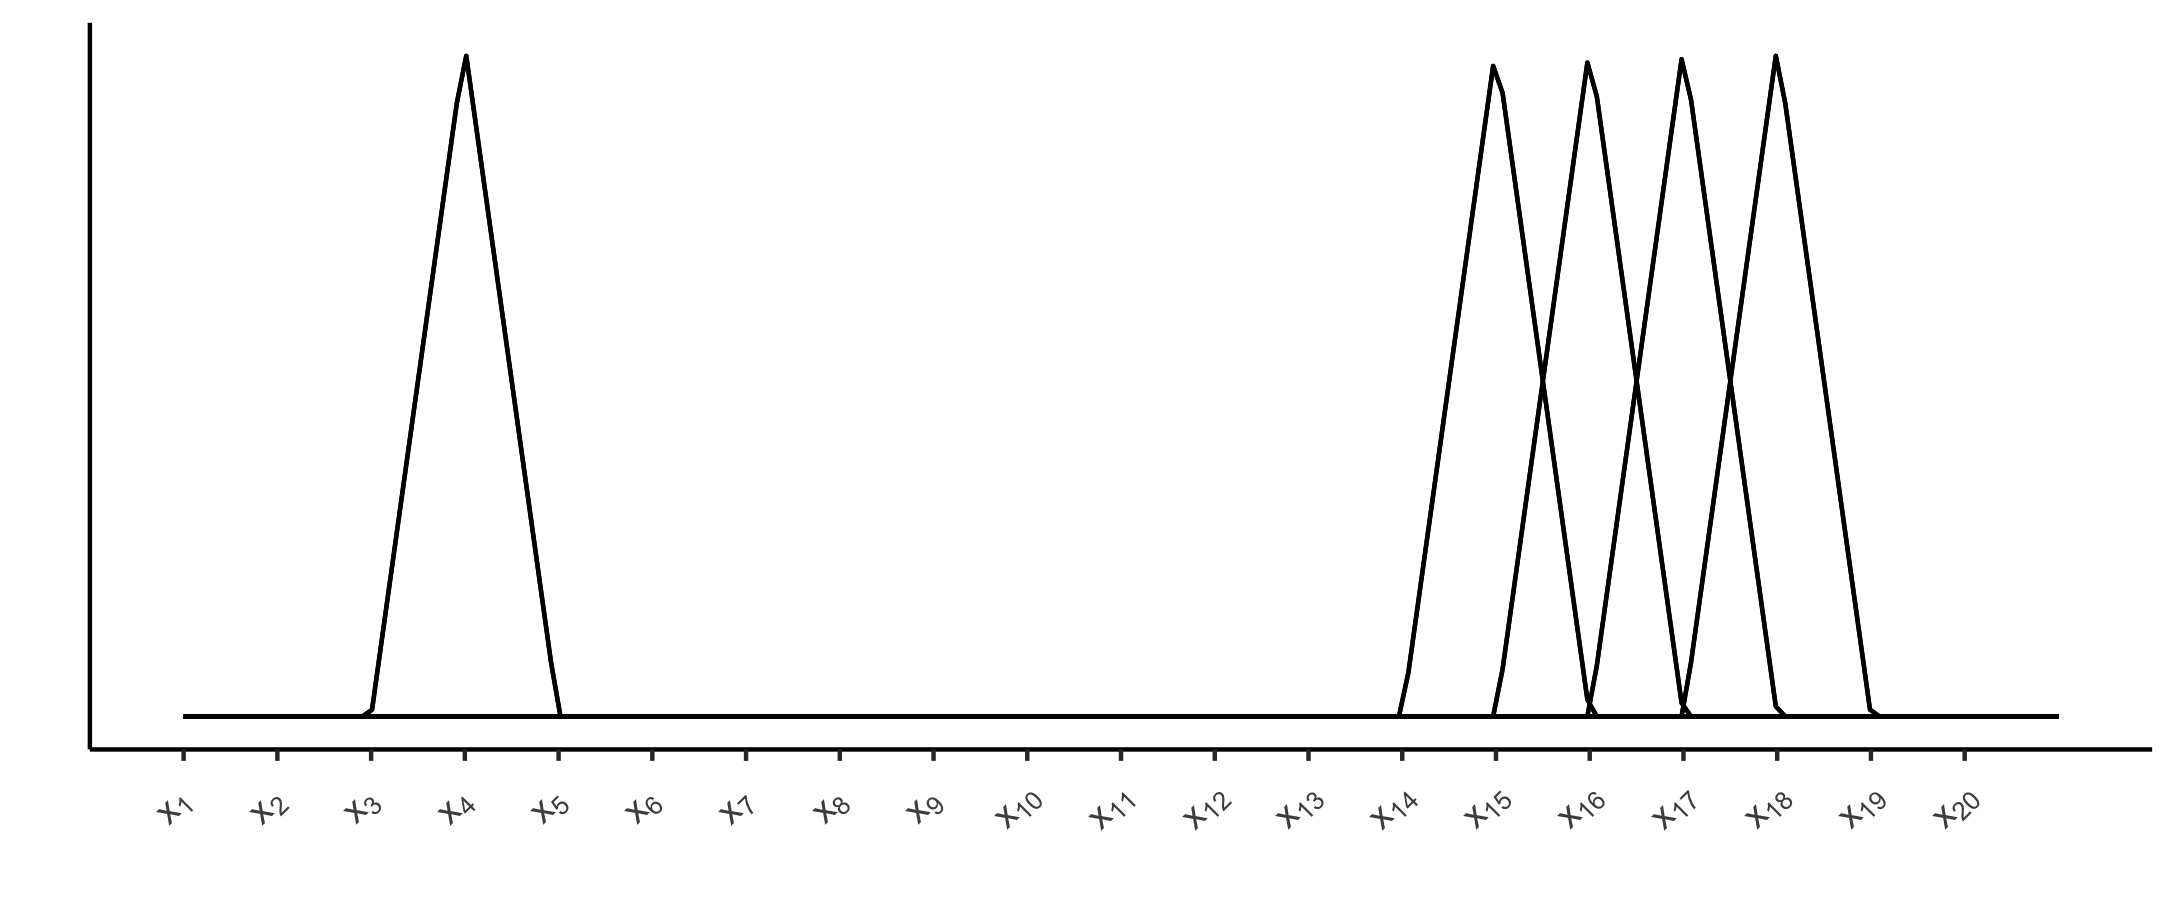
\includegraphics[width=0.75\textwidth]{img/uni_linear_bsplines}
 \caption{of degree 1} \label{fig:overlapping-linear-bsplines}
  \end{subfigure}
   \end{center}
  \hfill
  \begin{center}
 \begin{subfigure}[t]{0.75\textwidth}
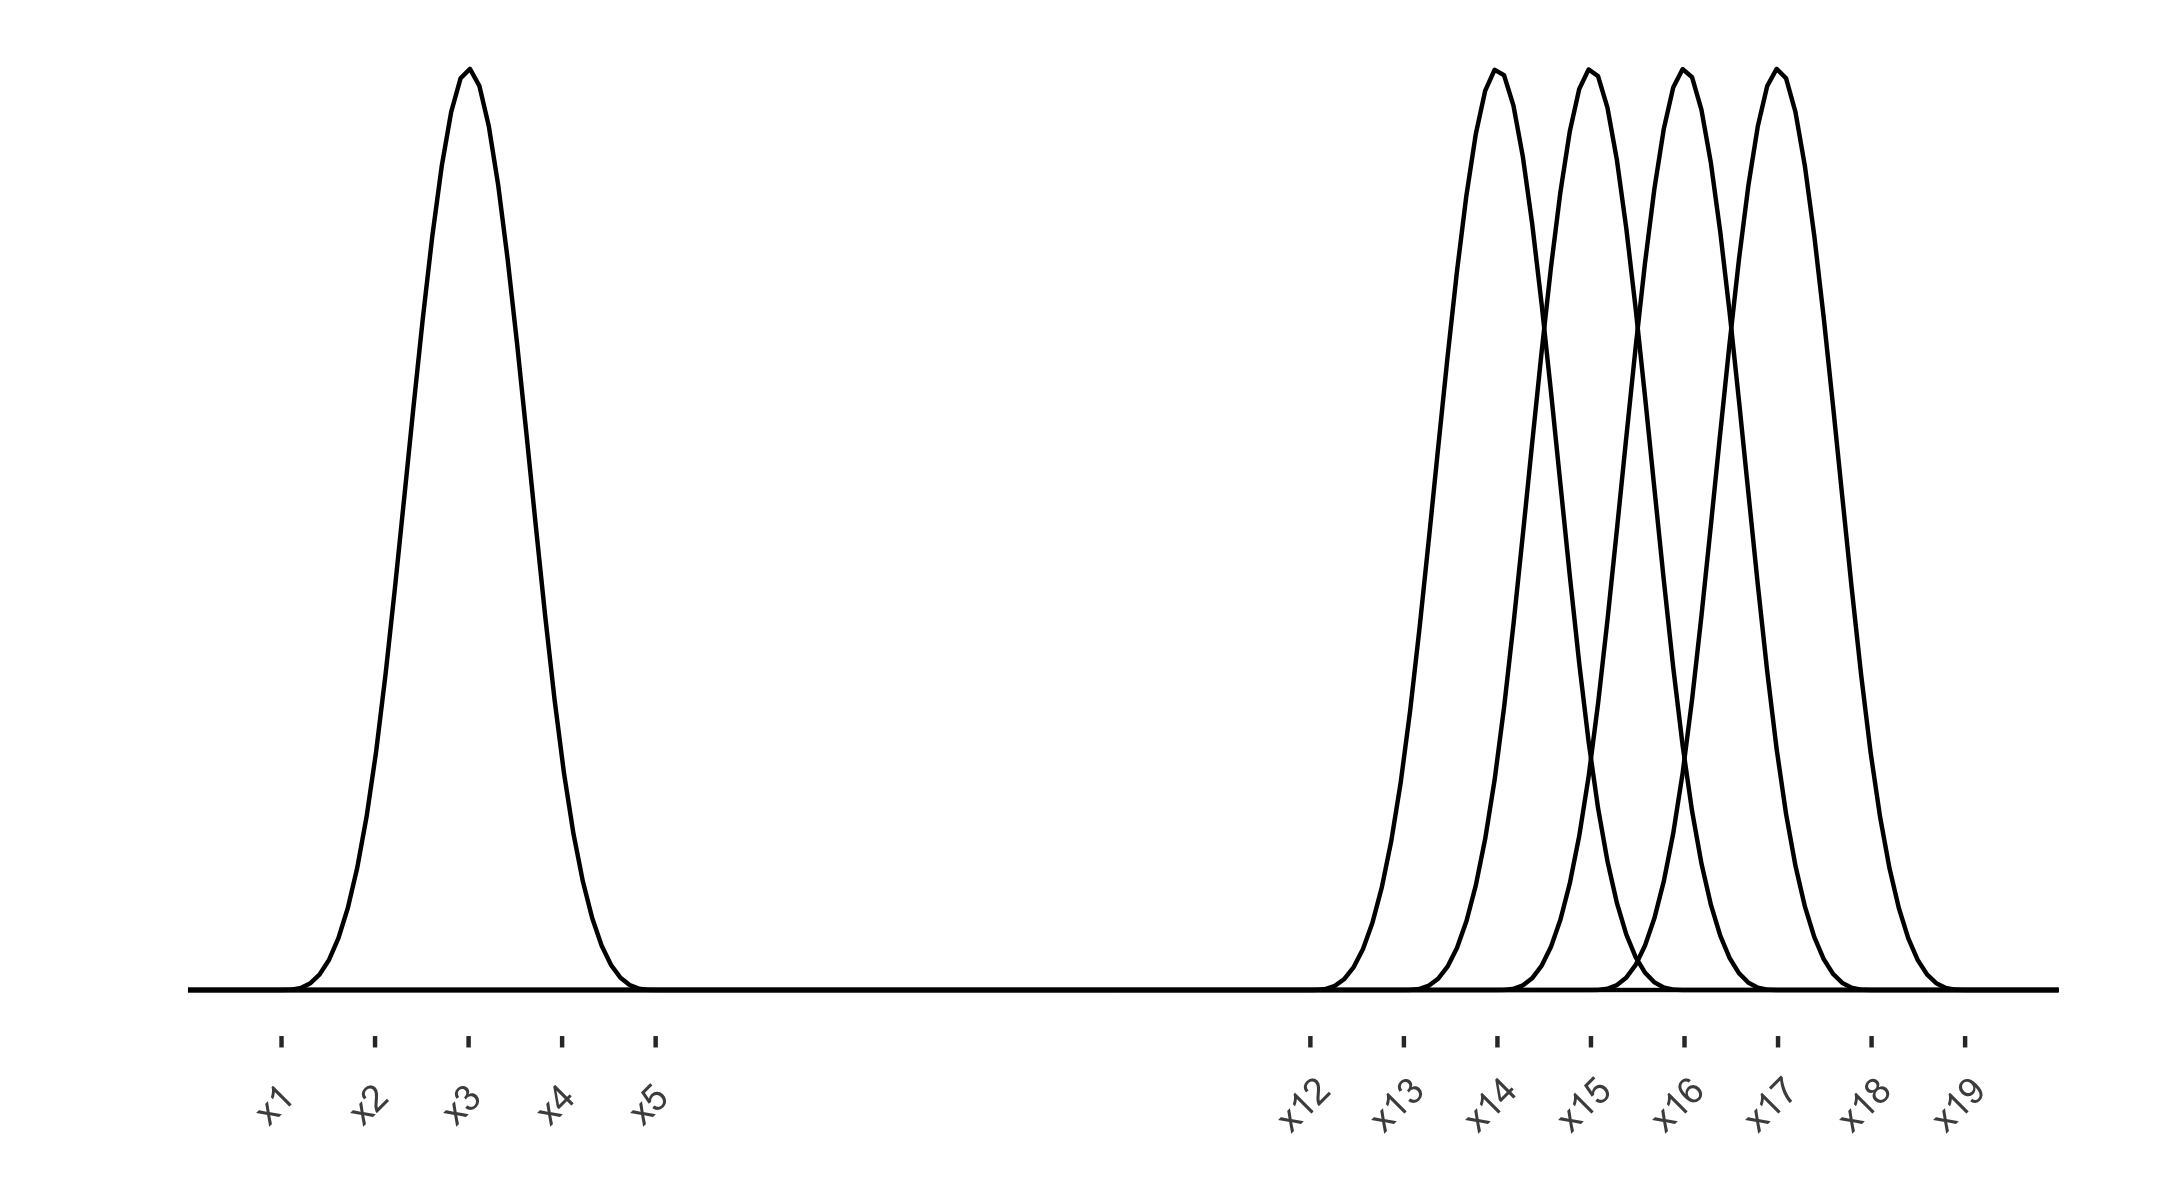
\includegraphics[width = \textwidth]{img/uni_cubic_bsplines}
 \caption{of degree 2}
\label{fig:overlapping-cubic-bsplines}
 \end{subfigure}
 \end{center}
\end{figure}

\begin{figure}[H]
  \centering
  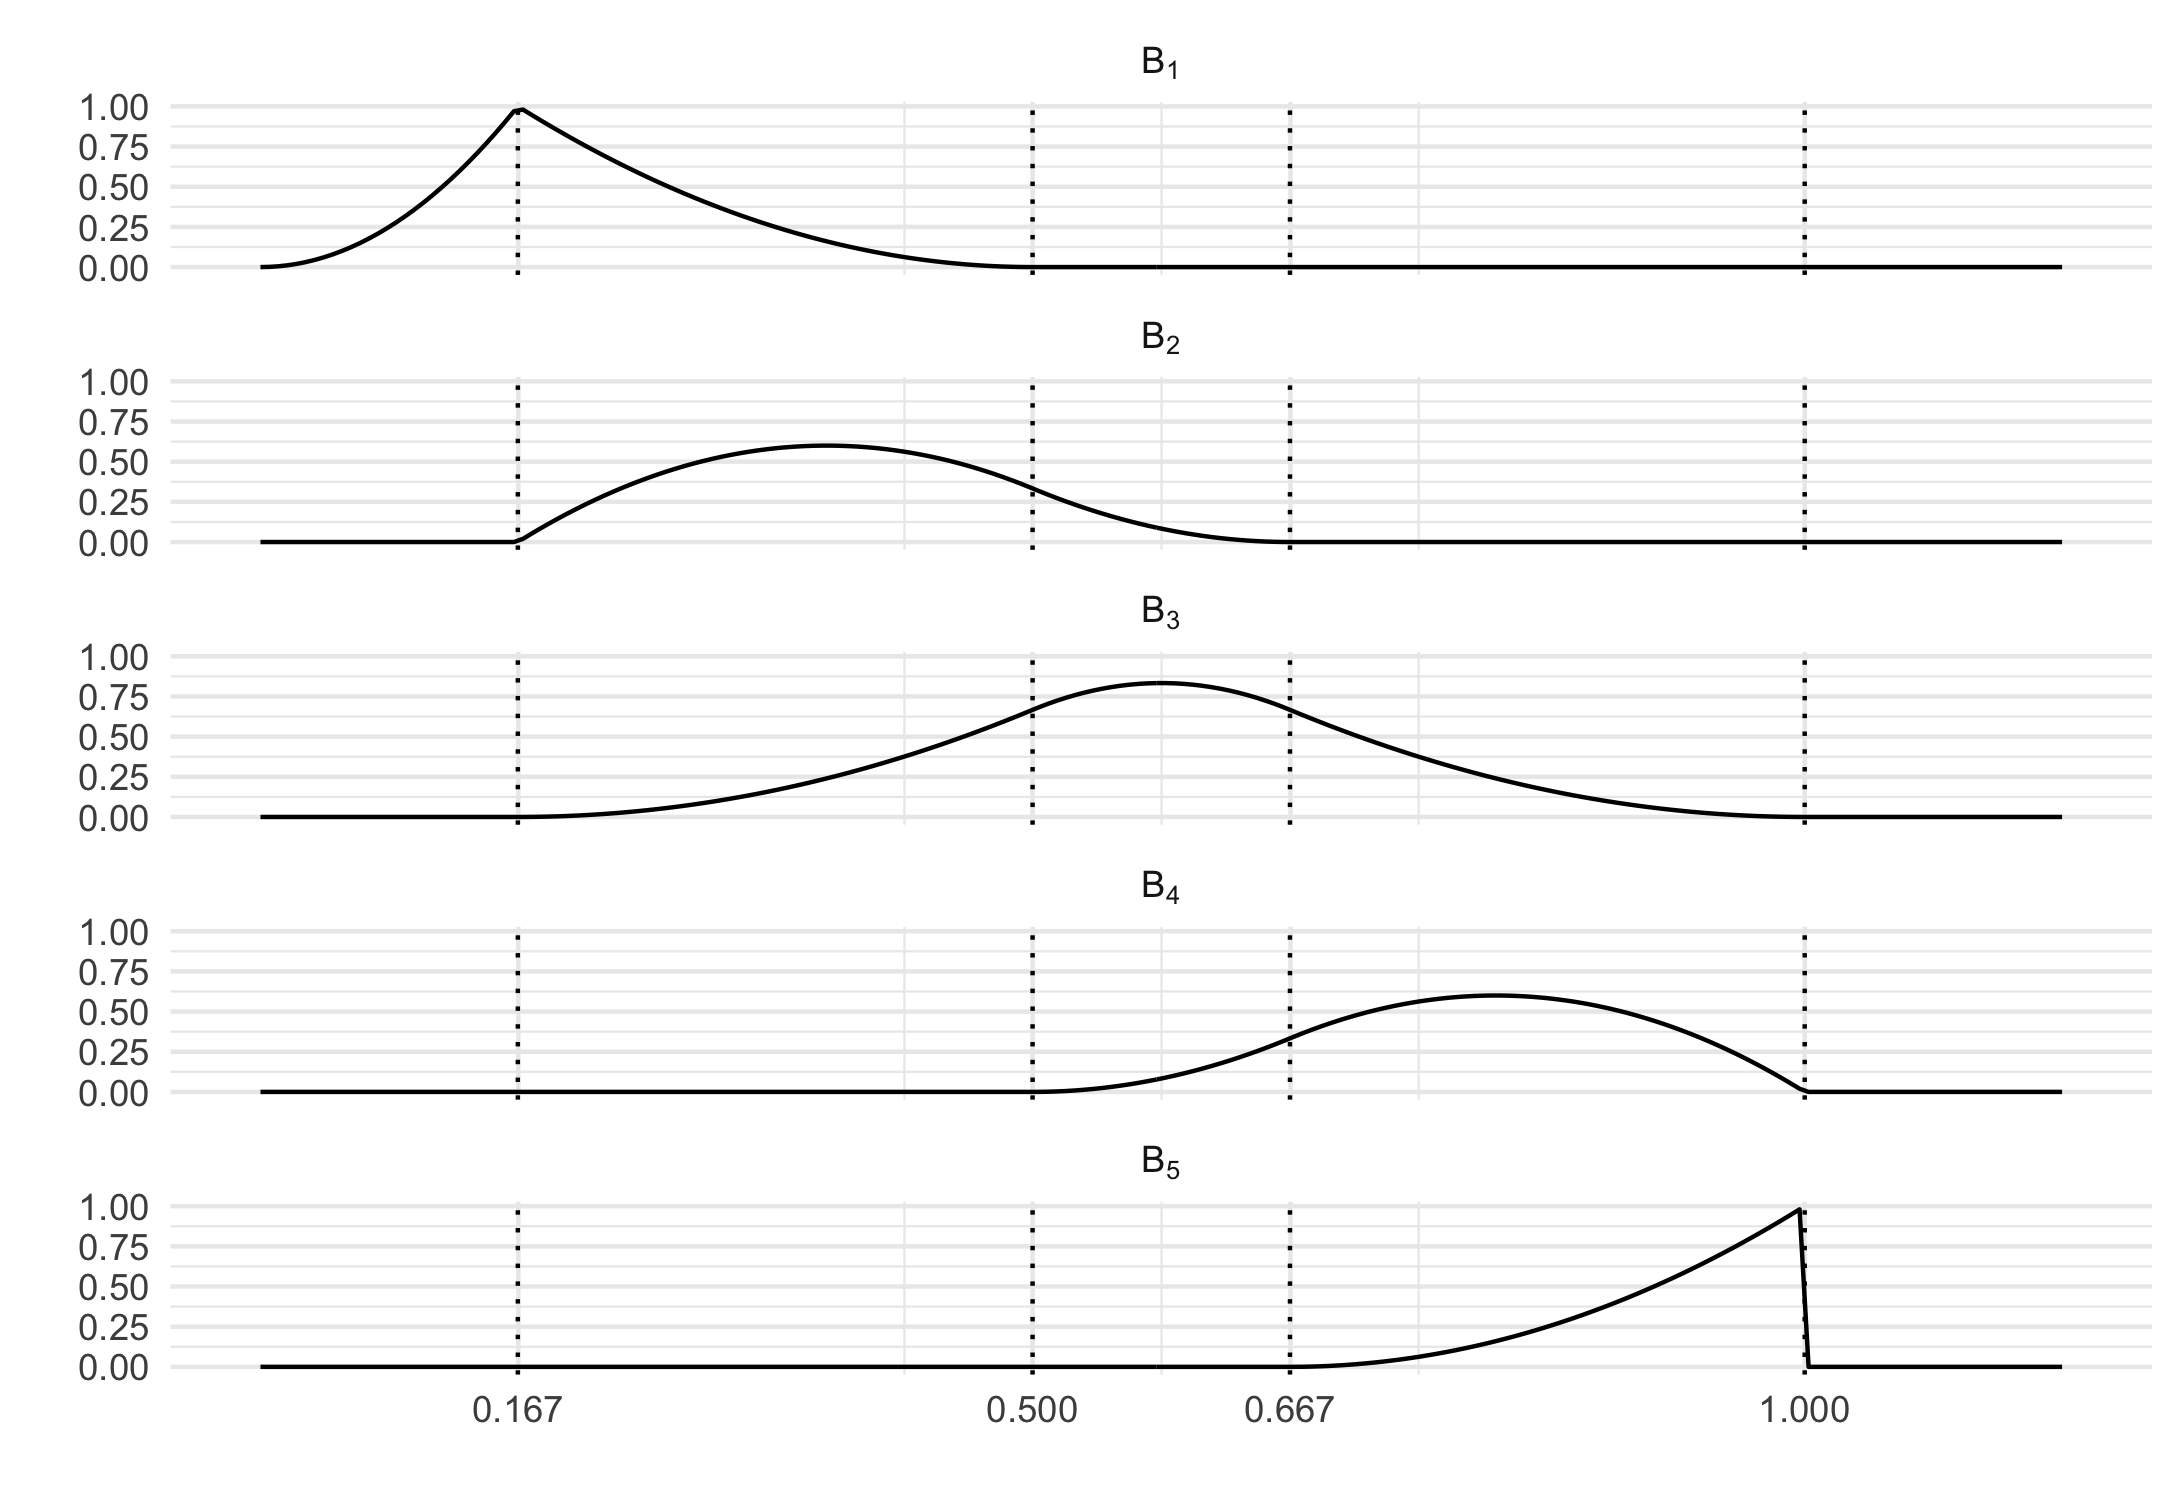
\includegraphics[width=5in,height=5in]{img/deboor_parabolic_bsplines}
  \caption{\textit{A set of parabolic B-splines corresponding to knot sequence  $\left\{\frac{1}{6}, \frac{1}{2}, \frac{2}{3}, 1\right\}$ }}\label{fig:parabolic-Bspline-basis}
\end{figure}


B-splines make attractive basis functions for nonparametric regression; a linear combination of, say, cubic B-splines gives a smooth curve. Once a B-spline basis is computed, their application is no more difficult than polynomial regression, and nearly seamless extension to two-dimensional smoothing is available with the use of tensor products. To construct a B-spline representation for $\phi$, we need to equip the $l$ and $m$ axes each with a B-spline basis: let

\[
B_{l,1}\left(l\right),\dots, B_{l,K_1}\left(l\right)  \mbox{ and } B_{m,1}\left(m\right),\dots, B_{m,K_2}\left(m\right)
\]
\noindent
denote the B-spline bases for $l$ and $m$, each having a set of equally spaced knots along their respective domain. It is worth noting that one is free to specify a different basis for each dimension either by using different order B-spline or, of course, using different numbers of knots. The tensor product basis functions
\begin{equation*}
T_{kk'}\left(l,m\right) = B_{l,k}\left(l\right){B}_{m,k'}\left(m\right)
\end{equation*}
\noindent
carve the $l$-$m$ domain into rectangles. Figure~\ref{fig:bicubic-bspline-function} shows a single $T_{kk'}$, where the marginal B-spline bases are of degree 2. Figure~\ref{fig:sparse_bicubic_BS_basis} shows a thinned tensor product basis $\left\{ T_{kk'} \right\}$; a portion of the basis was omitted to eliminate overlapping of the basis functions so that the reader can identify individual tensor products. Each ``hill'' in Figure~\ref{fig:sparse_bicubic_BS_basis} is associated with an unknown coefficient $\theta_{ij}$ which determines the height of the hill. For a given knot grid, we can approximate a surface, $\phi$, by

\begin{equation} \label{eq:tensor-product-bspline-expansion-phi}
\phi\left(l,m\right) = \sum_{i=1}^{k_1} \sum_{j=1}^{k_2} \theta_{ij} B_{l,i}\left(l\right) B_{m,j}\left(m\right). 
\end{equation}
\noindent
 By using rich B-spline bases for $l$ and $m$ alongside discrete difference penalties on the spline coefficients, we can achieve as much smoothness of the fitted function in both the $l$ and $m$ dimensions as desired. Fixing $\sigma^2$ as in (\ref{eq:penalized-joint-loglik-given-sigma}), we can define the estimator of $\phi$ as the minimizer of

\begin{equation} 
-2\ell_\phi + \lambda J\left(\phi\right) = \sum_{i=1}^N \sum_{j=2}^{m_i} \sigma^{-2}_{ij}\left( y_{ij} - \sum_{k<j} \phi\left(\bfv_{ijk}\right) y_{ik}  \right)^2 + \lambda J\left( \phi \right),
\end{equation} 
\noindent
where $J\left(\phi\right)$ penalizes the smoothness of the fitted function. 


\begin{figure}[H]
  \caption{\textit{ Tensor product of two cubic B-splines }}\label{fig:bicubic-bspline-function}
    \begin{center}
 \begin{subfigure}[t]{0.48\textwidth}
  \centering
  \includegraphics[width=\textwidth]{img/bicubic_basis_function}
  \end{subfigure}
 \begin{subfigure}[t]{.48\textwidth}
  \centering
\includegraphics[width=\textwidth]{img/bicubic_bspline_contour}
 \end{subfigure}
 \end{center}
\end{figure}


\begin{figure}[H]
  \centering
  \graphicspath{{img/}}
  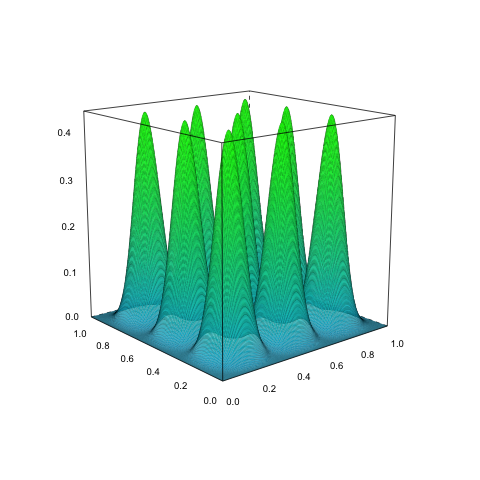
\includegraphics[width=5in,height=5in]{sparse_bicubic_basis.png}
  \caption{\textit{A subset of a full bivariate basis of cubic B-splines}}\label{fig:sparse_bicubic_BS_basis}
\end{figure}


%%%%%%%%%%%%%%%%%%%%%%%%%%%%%%%%%%%%%%%%%%%%%%%%%%%%%%%%%%%%%%%%%%%%%%%%%%%%%%%%%%%%%%%%%%%
%%%%%%%%%%%%%%%%%%%%%%%%%%%%%%%%%%%%%%%%%%%%%%%%%%%%%%%%%%%%%%%%%%%%%%%%%%%%%%%%%%%%%%%%%%%
%%%%%%%%%%%%%%%%%%%%%%%%%%%%%%%%%%%%%%%%%%%%%%%%%%%%%%%%%%%%%%%%%%%%%%%%%%%%%%%%%%%%%%%%%%%
%%%%%%%%%%%%%%%%%%%%%%%%%%%%%%%%%%%%%%%%%%%%%%%%%%%%%%%%%%%%%%%%%%%%%%%%%%%%%%%%%%%%%%%%%%%

\subsection{Difference penalties}

\cite{o1986statistical} was the first to propose using a rich B-spline basis alongside a penalty to restrict the flexibility of the fitted curve, like \citet{wahba1990spline} applying a penalty to the second derivative of the fitted curve (taking one-dimensional inputs):
\begin{equation} \label{eq:second-derivative-penalty}
J = \int_0^1 \left[ \phi^{\prime \prime}\right]^2.
\end{equation}

For a B-spline of the form
\[
\phi\left(v\right) = \sum\limits_{j=1}^k \theta_i B_j\left(v\right),
\]
one can derive a banded matrix $P$ using the properties of B-splines such that 
 \[
 J = \theta^\prime P \theta
 \] 
 \noindent
 where $\theta = \left(\theta_1,\dots, \theta_k\right)$ denotes the vector of B-spline basis coefficients. The $i$-$j^{th}$ element of the penalty matrix $P$ is given by
 \[
 p_{ij} = \int_0^1 B_i^{\prime \prime} B_j^{\prime \prime}.
 \]

The computation of $P$ is nontrivial and becomes very tedious when the third and fourth derivative are used as the roughness measure. \cite{wand2008semiparametric} extend O'Sullivan's work to higher order derivatives for general degree B-splines and derive an exact matrix algebraic expression for the penalty matrices. In the cubic case, the expression is a result of the application of Simpson's Rule applied to the inter-knot differences since each $B_i^{\prime \prime} B_j^{\prime \prime}$ is a piecewise quadratic function. The penalty may be written
 \[
 P = \left(B^{\prime \prime}\right)^\prime \textup{diag}\left(\omega \right) B^{\prime \prime}, 
 \]
 \noindent
 where $B^{\prime \prime}$ is the $3\left( k + 7 \right) \times \left( k + 4 \right)$ matrix with $i$-$j^{th}$ entry given by $B_j^{\prime \prime} \left(x_i^*\right)$, $x^*_i$ is the $i^{th}$ element of 
 
\[
\left( \phi_1,\frac{\phi_1+\phi_2}{2},\phi_2,\phi_2,\frac{\phi_2+\phi_3}{2},\phi_3,\dots,\phi_{k+7},\frac{\phi_{k+7}+\phi_{k+8}}{2},\phi_{k+8} \right),
\]
 \noindent
 and $\omega$ is the $3\left(k+7\right) \times 1$ vector given by
 
\begin{align*}
\omega &= \left( \frac{1}{6}\left(\Delta \phi \right)_1,\frac{4}{6}\left(\Delta \phi \right)_1, \frac{1}{6}\left(\Delta \phi \right)_1,\frac{1}{6}\left(\Delta \phi \right)_2, \frac{4}{6}\left(\Delta \phi \right)_2,  \right. \\
&\qquad   \left. {} \frac{1}{6}\left(\Delta \phi \right)_2 , \dots , \frac{1}{6}\left(\Delta \phi \right)_{n+7}, \frac{4}{6}\left(\Delta \phi \right)_{k+7}, \frac{1}{6}\left(\Delta \phi \right)_{k+7}  \right) \\
\end{align*}
\noindent
 where $\left(\Delta \phi \right)_j = \phi_{j+1}-\phi_j$. They generalize this to the case of any order penalty and present a table of formulas for constructing any arbitrary penalty matrix, $P$.  Alternatively, Eilers and Marx proposed replacing the derivative-based penalty (\ref{eq:second-derivative-penalty}) with a finite difference penalty on the B-spline coefficients. Using the properties of B-splines, it is straightforward to show that the difference penalty of order $d$ is a good discrete approximation to the integrated square of the $d^{th}$ derivative, so little is lost by using it in place of the derivative-based penalty. The difference penalty is simple to compute and can be handled mechanically for any order of the differences, and since it is easily appended to a goodness of fit measure (such as the log likelihood), it is feasible to evaluate the impact of different orders of the differences on the fitted model.  

\bigskip

The $d^{th}$ order difference penalty is given by 

\begin{equation} \label{eq:bspline-difference-penalty-1}
J_d\left( \phi \right) = \sum_{j=d}^n \left(\Delta^d \theta_j\right)^2,
\end{equation} 
\noindent
Let $D_d$ denote the matrix difference operator:

\[
D_d\theta = \Delta^d \theta,
\]
\noindent
where $\Delta \theta_j = \theta_j - \theta_{j-1}$, and $\Delta^2 \theta_j = \Delta\left(\Delta \theta_j\right) = \theta_j - 2\theta_{j-1} + \theta_{j-2}$. In general,
\begin{equation*}
\Delta^d \theta_j = \Delta\left(\Delta^{d-1} \theta_j \right).
\end{equation*} 
\noindent
Then, \ref{eq:bspline-difference-penalty-1} can be written in terms of the squared norm of the difference operator applied to the vector of B-spline coefficients:
\begin{align} 
\begin{split} \label{eq:bspline-difference-penalty-2}
J_d\left( f \right) &= \vert \vert D_d\theta \vert \vert^2 \\
&= \theta^\prime P_d \theta
\end{split}
\end{align}
\noindent
where $P_d = D_d^\prime D_d$.  To examine the connection between the second-derivative penalty to the penalty on second-order differences of the B-spline coefficients, we only need to employ straightforward calculus and exploit the recursive property of the B-spline basis functions. Consider a function $f$ defined as a linear combination of $k$ cubic B-spline basis functions, $f = \sum_{i = 1}^k \theta_i B_{i,3}$. Then the traditional smoothness penalty applied to $f$ is given by

\begin{equation*} 
\int_0^1 \left[ f^{\prime \prime}\right]^2\ = \int_{0}^{1} \left\{ \sum\limits_{j=1}^k  \theta_j B_{j,3}^{\prime \prime} \right\}^2.
\end{equation*}
\noindent
The derivative properties of B-splines permits this to be written as 

\begin{equation*} \label{eq:second-derivative-bspline-penalty}
\int_0^1 \left[ f^{\prime \prime}\right]^2\ =  \int_{0}^{1}  \bigg[ \sum\limits_{i=1}^k \sum\limits_{j=1}^k \Delta^2 \theta_i \Delta^2 \theta_j B_{i,1}B_{j,1}\bigg]. 
\end{equation*}
\noindent
Most of the cross products of $B_{i,1}$ and $B_{j,1}$ vanish since B-splines of degree 1 only overlap when $j$ is $i-1$, $i$, or $i+1$. Thus, we have that

\begin{align}
\begin{split}
\int_0^1 \left[ f^{\prime \prime}\right]^2  = {} &  \int_0^1 \bigg[ \left( \sum\limits_{j=1}^k   \Delta^2 \theta_j  B_j \right)^2  + 2 \sum_{j}\Delta^2 \theta_j\Delta^2 \theta_{j-1}B_{j,1}B_{j-1,1} \bigg]\\ 
= {} & \sum \limits_{j=1}^k  \left( \Delta^2\theta_j \right)^2 \int_0^1 B_{j,1}^2\ + 2 \sum\limits_{j=1}^k \Delta^2 \theta_j\Delta^2 \theta_{j-1} \int_0^1 B_{j,1}B_{j-1,1} 
\end{split}
\end{align}
\noindent
which can be written as

\begin{equation} \label{eq:derivative-penalty-difference-penalty-connection}
\int_0^1 \left[ f^{\prime \prime}\right]^2  = c_1 \sum\limits_{j=2}^k \left( \Delta^2 \theta_j\right)^2 + c_2 \sum\limits_{j=3}^n \Delta^2 \theta_j\Delta^2 \theta_{j-1}
\end{equation}
\noindent
Given a set of equidistant knots, the constants $c_1$ and $c_2$ are given by
\begin{equation}
\begin{split}
c_1 & =   \int_0^1 B_{j,1}^2\\\
c_2 & = \int_0^1 B_{j,1}B_{j-1,1}.
\end{split}
\end{equation}


This establishes that traditional smoothness penalty on the squared second derivative can be written as a linear combination of a penalty on the second-order differences of the B-spline coefficients \ref{eq:bspline-difference-penalty} and the sum of the cross products of neighboring second differences. The second term in \ref{eq:derivative-penalty-difference-penalty-connection} leads to a complex objective function when minimizing the penalized likelihood, where seven adjacent spline coefficients occur, as opposed to five if only the first term in \ref{eq:derivative-penalty-difference-penalty-connection} is used in the penalty. The added complexity is a consequence of overlapping B-splines, which quickly increases when using higher order differences and higher order B-splines. We can seamlessly augment the likelihood with the difference penalty to achieve smooth fitted functions without the complexity posed by the derivative-based penalty.

\bigskip

A smoother sequence of coefficients leads to a smoother curve, as illustrated in Figure~\ref{fig:increasing-lambda-pspline-fits}.  The relationship between P-spline curves and their coefficients is easily characterized if we consider the coefficients as the skeleton of the function, and draping the B-splines over them puts the flesh on the bones. As long as the coefficient sequence is smooth, the number of basis functions (and coefficients) is unimportant since the penalty ensures the smoothness of the skeleton and that the fitting procedure is well-conditioned.  Unless computational constraints are of concern, which is possible with large models, it is prudent to use even more B-splines.  Figure~\ref{fig:overcomplete-pspline-basis} illustrates this utility of the penalty for simulated data; there are $M=10$ observations and $60$ cubic B-splines. 

\begin{figure}[H] 
\begin{subfigure}{.5\textwidth}
  \centering
   \graphicspath{{img/}}
  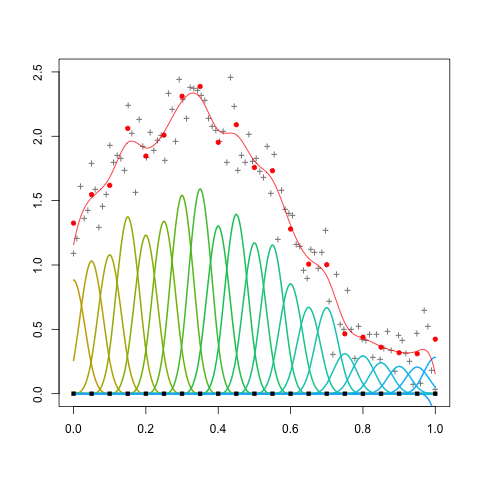
\includegraphics[scale=0.5]{pspline_pord2_xsmall_lambda.png}
  \label{fig:pspline_small_lambda}
\end{subfigure}
\begin{subfigure}{.5\textwidth}
  \centering
   \graphicspath{{img/}}
  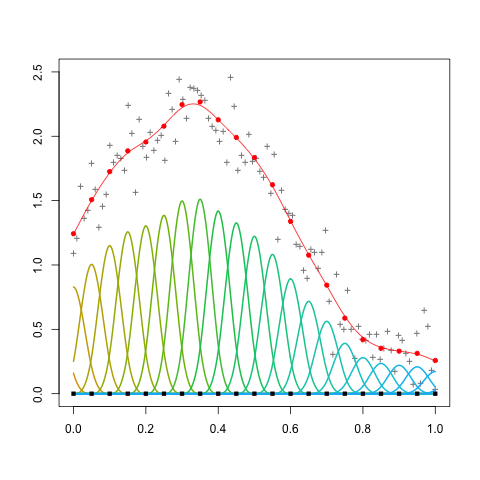
\includegraphics[scale=0.5]{pspline_pord2_small_lambda.png}
  \label{fig:pspline_small_lambda}
\end{subfigure}
\begin{subfigure}{.5\textwidth}
  \centering
   \graphicspath{{img/}}
  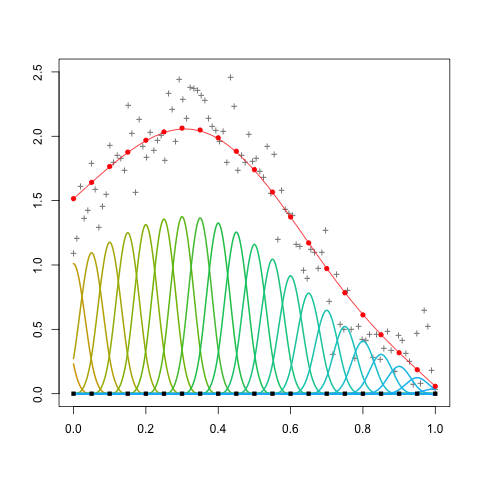
\includegraphics[scale=0.5]{pspline_pord2_medium_lambda.png}
  \label{fig:pspline_small_lambda}
\end{subfigure}
\begin{subfigure}{.5\textwidth}
  \centering
   \graphicspath{{img/}}
  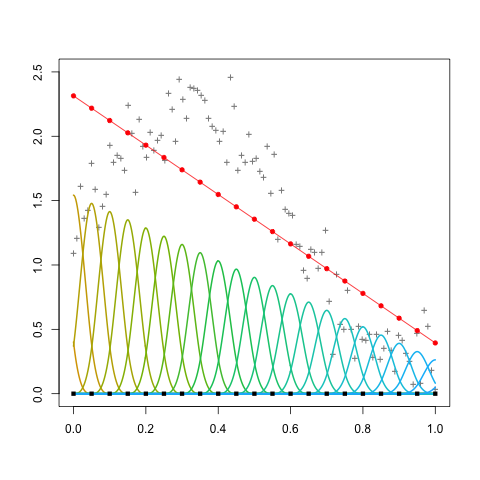
\includegraphics[scale=0.5]{pspline_pord2_large_lambda.png}
  \label{fig:pspline_small_lambda}
\end{subfigure}
\caption{\textit{Illustration of the impact of the second order difference penalty. The number of B-splines used is the same in each plot, with the value of the penalty parameter increasing from left to right and top to bottom across each plot. The fitted curve in the upper left plot is the most ``wiggly'' of any of the fits, as the penalty plays the weakest roll in the fitted coefficients there. The red circles are the values of each of the B-spline coefficients; as the penalty increases, they form as smoother sequence as we move across the four plots, which results in a smoother fitted function. As the penalty parameter approaches infinity, the fit approaches a linear function as shown in the bottom right plot.}}
\label{fig:increasing-lambda-pspline-fits}
\end{figure}

\begin{figure}[H] 
\centering
\graphicspath{{img/}}
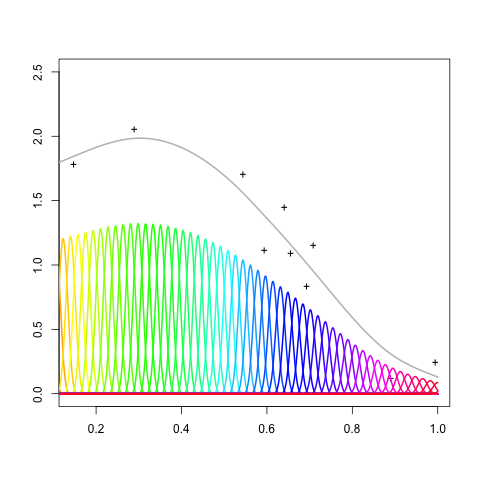
\includegraphics[scale=0.75]{pspline_10obs_60_basis_functions.png}
\caption{\textit{P-spline smoothing of 10 observations using 60 B-spline basis functions.}} \label{fig:overcomplete-pspline-basis}
\end{figure}

P-splines can fit polynomial data exactly - if they true underlying function to be estimation is a polynomial of degree $k$ in $l$, then B-splines of degree $k$ or higher will fit the data exactly. The proof of this requires a bit of mathematical labor and is left to Appendix~\ref{chapter-3-appendix}. Additionally, the limiting P-spline fit approaches a polynomial as the smoothing parameter tends to infinity.  As $\lambda \rightarrow \infty$, under a difference penalty of order $d$, the fitted function will approach a polynomial of degree $d-1$ as long as the degree of the B-splines is greater than or equal to $k$. Figure~\ref{fig:PS-difference-order-demo} demonstrates the impact of the order of the penalty on the fitted function as the smoothing parameter increases. To verify this mathematically, we need to use the relationship between the differenced coefficient sequence and the derivative of a B-spline - see Appendix~\ref{chapter-3-appendix}. Consider using the second-order difference penalty; when $\lambda$ is large, the penalty dominates the P-spline objective function defined in \ref{eq:S_pen_varying_intercept_model}, so that the minimizer $\theta$ must be such that $\sum_{j=3}^k\left(\Delta^2\theta_j\right)^2$ is close to zero. Consequently, each of the individual second differences must also be nearly zero, and thus the second derivative of the fitted function must be close to zero over the entire domain.

\begin{figure}[H]
\begin{subfigure}{.5\textwidth}
  \centering
   \graphicspath{{img/}}
  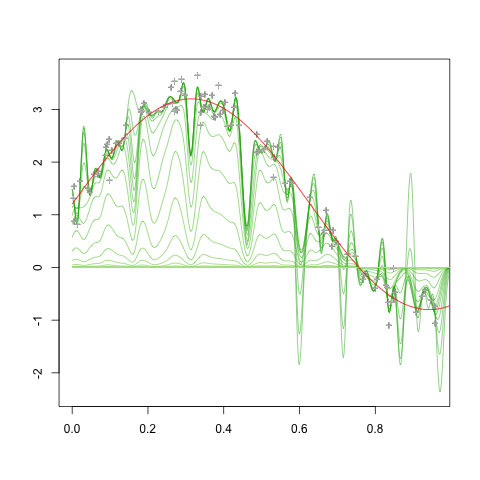
\includegraphics[scale=0.5]{PS_penalty_section_figure_6_order_0.png}
  %\label{fig:pspline_small_lambda}
\caption{$d=0$ }
\end{subfigure}
\begin{subfigure}{.5\textwidth}
  \centering
   \graphicspath{{img/}}
  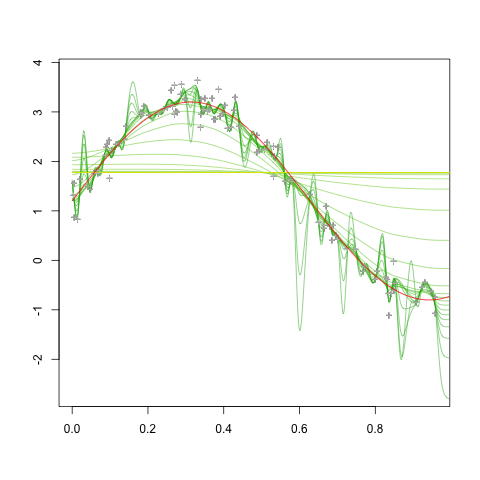
\includegraphics[scale=0.5]{PS_penalty_section_figure_6_order_1.png}
 % \label{fig:pspline_small_lambda}
\caption{$d=1$}
\end{subfigure}
\begin{subfigure}{.5\textwidth}
  \centering
   \graphicspath{{img/}}
  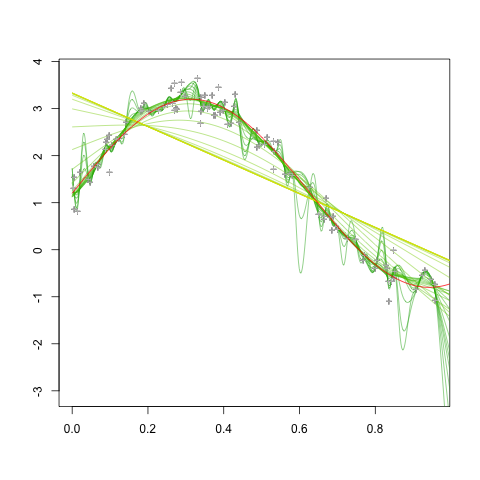
\includegraphics[scale=0.5]{PS_penalty_section_figure_6_order_2.png}
  %\label{fig:pspline_small_lambda}
\caption{$d=2$}
\end{subfigure}
\begin{subfigure}{.5\textwidth}
  \centering
   \graphicspath{{img/}}
  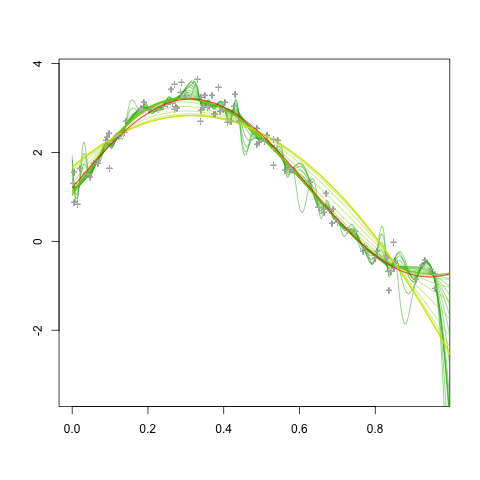
\includegraphics[scale=0.5]{PS_penalty_section_figure_6_order_3.png}
  %\label{fig:pspline_small_lambda}
\caption{$d=3$}
\end{subfigure}
\caption{\textit{Illustration of the impact of the order of the difference penalty. The number of B-splines used is the same in each plot, with the penalty parameter varying from across the same grid of values. The fitted curves in the upper left plot correspond to the difference penalty of order $0$, where $\vert D_0 \theta \vert^2 = \sum_{i} \theta_i^2$, analogous to ridge regression using the B-spline basis as regression covariates. The fitted curves approach polynomials of degree $d-1$ as $\lambda \rightarrow \infty$.}}
\label{fig:PS-difference-order-demo}
\end{figure}


%%%%%%%%%%%%%%%%%%%%%%%%%%%%%%%%%%%%%%%%%%%%%%%%%%%%%%%%%%%%%%%%%%%%%%%%%%%%%%%%%%%%%%%%%%%
%%%%%%%%%%%%%%%%%%%%%%%%%%%%%%%%%%%%%%%%%%%%%%%%%%%%%%%%%%%%%%%%%%%%%%%%%%%%%%%%%%%%%%%%%%%
%%%%%%%%%%%%%%%%%%%%%%%%%%%%%%%%%%%%%%%%%%%%%%%%%%%%%%%%%%%%%%%%%%%%%%%%%%%%%%%%%%%%%%%%%%%
%%%%%%%%%%%%%%%%%%%%%%%%%%%%%%%%%%%%%%%%%%%%%%%%%%%%%%%%%%%%%%%%%%%%%%%%%%%%%%%%%%%%%%%%%%%
%%%%%%%%%%%%%%%%%%%%%%%%%%%%%%%%%%%%%%%%%%%%%%%%%%%%%%%%%%%%%%%%%%%%%%%%%%%%%%%%%%%%%%%%%%%
%%%%%%%%%%%%%%%%%%%%%%%%%%%%%%%%%%%%%%%%%%%%%%%%%%%%%%%%%%%%%%%%%%%%%%%%%%%%%%%%%%%%%%%%%%%
%%%%%%%%%%%%%%%%%%%%%%%%%%%%%%%%%%%%%%%%%%%%%%%%%%%%%%%%%%%%%%%%%%%%%%%%%%%%%%%%%%%%%%%%%%%
%%%%%%%%%%%%%%%%%%%%%%%%%%%%%%%%%%%%%%%%%%%%%%%%%%%%%%%%%%%%%%%%%%%%%%%%%%%%%%%%%%%%%%%%%%%



\subsubsection{Construction of the solution $\hat{\phi}$}

To extend the use of the difference penalty (\ref{eq:bspline-difference-penalty-1}) to the bivariate setting, the only necessary modification to the one-dimensional differencing procedure is the addition of a second difference penalty, one for each variable $l$ and $m$. The explicit form of the minimizer of the penalized log likelihood is available, but for exposition, we first need to establish some notation. The smooth varying coefficient function $\phi$ evaluated at a $n_1 \times n_2$ grid of points over the $l \times m$ plane may be written 

\begin{equation*} 
\vphistar = B_2 \Theta B'_1
\end{equation*}
\noindent 
where $B_1$ is the $n_1 \times k_1$ matrix with $i^{th}$ column equal to the $i^{th}$ B-spline basis function for $l$ evaluated at the grid points $l_1,\dots l_{n_1}$,  $B_2$ is the $n_2 \times k_2$ matrix with $j^{th}$ column equal to the $j^{th}$ B-spline basis function for $m$ evaluated at the grid points $m_1,\dots m_{n_2}$. The matrix $\Theta$ denotes the $k_1 \times k_2$ matrix of tensor product coefficients, with elements $\theta_{ij}$. Smoothing $\phi$ in the $l$ direction can be achieved by applying a difference penalty to the rows of $\Theta$, and similarly in the $m$ direction by applying a difference penalty to the columns. We take $\phi_\lambda$ to be the minimizer of 

\begin{align} 
\begin{split}\label{eq:folded-difference-penalty-log-likelihood}
&-2\ell + J_\theta \left(\phi\right) = \sum_{i=1}^N \sum_{j=2}^{m_i} \sigma^{-2}\left({t_{ij}}\right) \left(y_{ij} - \sum_{k=1}^{j-1} \left( \sum_{r=1}^{k_1} \sum_{c=1}^{k_2} \theta_{rc} B_r\left(l_{ijk}\right)B_c\left(m_{ijk}\right)\right)y_{ik} \right)^2 \\ 
&\phantom{{}-2\ell + J_\theta \left(\phi\right) = {}} + \lambda_1 \sum_{r=1}^{k_1} \vert D_{d_{\ms l}} \theta_{r \cdot} \vert^2 + \lambda_2 \sum_{c=1}^{k_2} \vert D_{d_{\ms m}} \theta_{\cdot c} \vert^2.
\end{split}
\end{align}
\noindent
where $\theta_{r \cdot}$ and $\theta_{\cdot c}$ denote the $r^{th}$ row and $c^{th}$ column of $\Theta$, respectively. The first term in\ref{eq:folded-difference-penalty-log-likelihood} imposes a difference penalty of order $d_{\ms l}$ on the rows of the coefficient matrix while the second term places a difference penalty (of possible different order $d_{\ms m}$) on the columns. We give each direction its own smoothing parameter to permit anisotropic smoothing; however, one could opt to use a single smoothing parameter for both directions and dodge the added work of optimizing the amount of smoothing with two separate parameters. Figure~\ref{fig:2d_PS_penalty_demo} shows a simple demonstration of the result of heavy column penalization (left) and heavy row penalization (right) under a second order difference penalty on each row and each column for large values of the smoothing parameters $\lambda_1$ and $\lambda_2$. The figure demonstrates that the limiting behavior of each row (column) is linear, but the resulting surface may exhibit slope reversals from one row (column) to the next. 

\begin{figure}[H] 
 \begin{subfigure}{.48\textwidth}
  \centering
   \graphicspath{{img/}}
 \includegraphics[scale=0.5]{"model selection/effective dimension/2d_PS_section_figure1_big_col_lambda"}
 \caption{\textit{heavy column penalty}}
 \label{fig:2D_PS_big_col_penalty}
 \end{subfigure}
 \begin{subfigure}{.48\textwidth}
  \centering
   \graphicspath{{img/}}
  \includegraphics[scale=0.5]{"model selection/effective dimension/2d_PS_section_figure1_big_row_lambda"}
 \caption{\textit{heavy row penalty}}
\label{fig:2D_PS_big_row_penalty}
 \end{subfigure}
 \caption{\textit{Nine cubic B-spline tensor products with heavy linear column penalty and heavy linear row penalty}}\label{fig:2d_PS_penalty_demo}
\end{figure}

\vspace{0.5cm}

The penalized log likelihood is quadratic in $\theta = \left(\theta_{11}, \dots, \theta_{k_1, k_2} \right)'$, and computation is quite simple if we express the coefficient matrix in ``unfolded'' notation. This allows us to express the varying coefficient function at the observed within-subject pairs of observation times as in the usual multiple regression form:

\begin{equation*}
\mbox{vec}\left\{\phi\left( \bfv \right)\right\} = B \theta
\end{equation*}
\noindent
Stacking the columns of $\Theta$ gives the vectorized coefficient matrix $\theta = \mbox{vec}\left( \Theta \right)$. The $\vert V \vert \times k_1 k_2$ tensor product basis $B$ is constructed from the tensor product of the marginal B-spline bases defined in \citet{eilers2006fast} as the \textit{row-wise Kronecker product} of the individual bases:

\begin{equation} \label{eq:rowwise-kronecker-product}
B = B_2 \square B_1 = \left( B_2 \otimes 1^\prime_{k_2} \right) \odot \left(1^\prime_{k_1} \otimes  B_1  \right).
\end{equation}
\noindent
The operator $\odot$ denotes the element-wise matrix product; $1_{k_1}$ ($1_{k_2}$) denotes the column vector of ones having length $k_1$ ($k_2$.) The operations in \ref{eq:rowwise-kronecker-product} construct $B$ such that the $i^{th}$ row of $B_2\square B_1$ is the Kronecker product of the corresponding rows of $B_2$ and $B_1$. The penalty in \ref{eq:folded-difference-penalty-log-likelihood} can also be compactly expressed:

\begin{equation*} \label{eq:tensor-product-penalty}
\lambda_1 \vert \vert P_1 \theta \vert \vert^2 + \lambda_m \vert \vert P_2 \theta \vert\vert^2
\end{equation*}
\noindent
where $P_1 = I_{k_2} \otimes D'_{d_{\ms l}} D_{d_{\ms l}} $ and $P_2 =  D'_{d_{\ms m}} D_{d_{\ms m}} \otimes I_{k_1}$. We define $Y$, the vector of stacked subject-specific vectors,  as before, and the matrix $X$ of autoregressive covariates as previously (\ref{eq:ar-design-matrix-1}) so that \ref{eq:folded-difference-penalty-log-likelihood} can be written in matrix form as

\begin{equation} \label{eq:tensor-pspline-objective-function}
-2L + J_\theta\left(\phi\right) = \left( Y - XB\theta\right)^\prime D^{-1}\left( Y - XB\theta\right)  + \lambda_1\vert\vert P_1 \theta \vert\vert^2 + \lambda_2 \vert\vert P_2 \theta\vert \vert^2,
\end{equation}
\noindent
with $\hat{\theta}$ solving the system of equations 
\begin{equation} \label{eq:tensor-pspline-normal-equations}
\left[ \left(XB\right)^\prime D^{-1} XB +  \lambda_1 P_1+ \lambda_2 P_2\right]\theta = \left(X B\right)^\prime D^{-1}Y.
\end{equation}
\noindent
From \ref{eq:tensor-pspline-normal-equations}, we note that the system of equations depends on basis coefficients remains fixed at $k_1 k_2$, even as the number of observations increases. The grid of regression coefficients can be recovered by arranging the elements of $\hat{\theta}$ into a matrix of $k_1$ columns having length $k_2$. The vector of fitted values is given by 

\begin{align*}
\hat{Y} &= X \left[ \left(XB\right)^\prime D^{-1} XB +  \lambda_1 P_1+ \lambda_2 P_2\right] \left(X B\right)^\prime D^{-1}Y\\
&= AY
\end{align*}
\noindent
where $A = X \left[ \left(XB\right)' D^{-1} XB +  \lambda_1 P_1+ \lambda_2 P_2\right] \left(X B\right)' D^{-1}$ is the ``smoothing'' matrix, analogous to the smoothing matrix $\tilde{A}$ (\ref{eq:smoothing-matrix-A-tilde}) for the smoothing spline estimator in Chapter 2. Its use in smoothing parameter selection and model tuning is similar to the reproducing kernel Hilbert space framework, which we will discuss in the next section.

\bigskip

This recipe for constructing a tensor product basis for $\phi$ is an easy and convenient way to construct a two-dimensional basis for a bivariate function with domain corresponding to the unit square. However, the domain autoregressive coefficient function, $\phi$, lies on the lower triangle of the unit square $0 < s < t < 1$:

\begin{figure}[H] \label{fig:triangle-domain}
    \graphicspath{{img/}}
 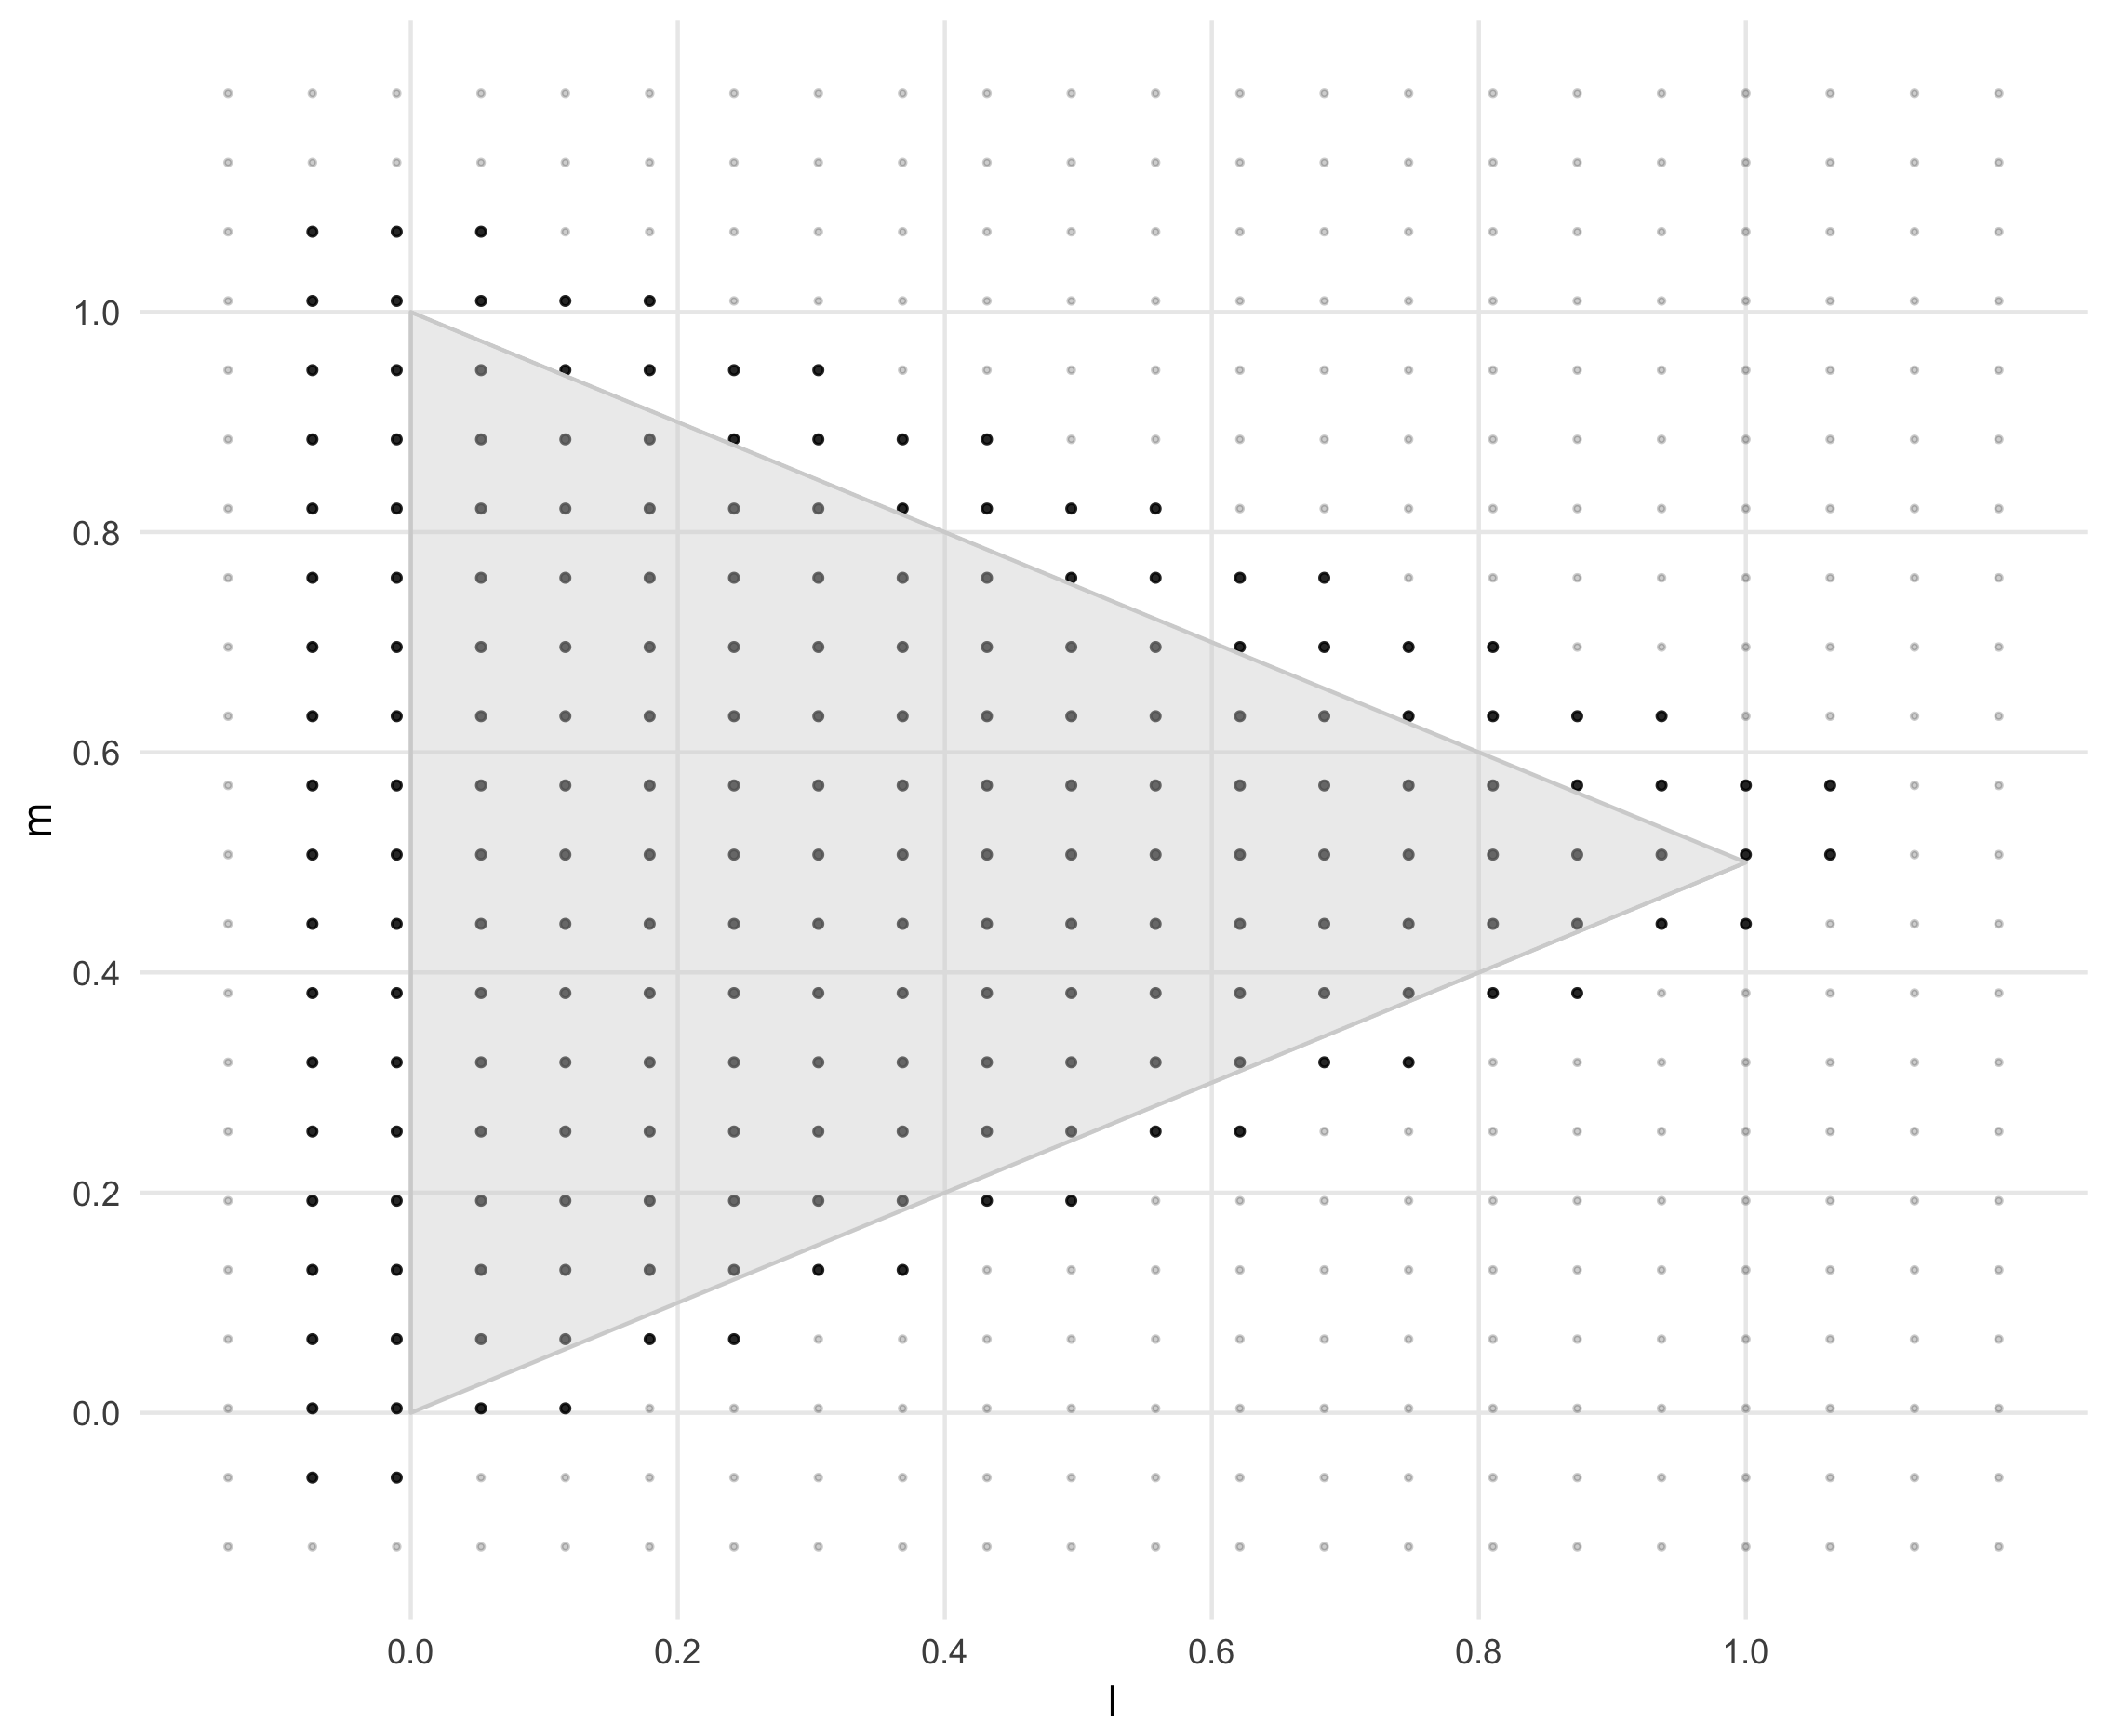
\includegraphics[scale=0.2]{knot-removal-on-triangle-domain.png}
 \caption{$\frac{l}{2} < m < 1 - \frac{l}{2}, \quad 0 < l < 1.$}
 \end{figure}


When the tensor product basis is constructed on the regular grid defined by the cartesian product of the knots of the marginal bases $B_1$ and $B_2$, a large number of basis functions anchored are at knots near which we have no data, so there is little information about the corresponding basis coefficient. As a result, the resulting tensor product matrix can be ill-conditioned and solving (\ref{eq:tensor-pspline-normal-equations}) results in singularities. In this case, the quality of the estimator can suffer terribly. To correct for this instability, one can simply remove the knots corresponding to tensor products functions which do not overlap with the function domain from the basis, $B$, and trimming the penalty matrices $P_1$ and $P_2$ as needed. With the trimmed basis and penalties, optimization can be carried out as previously discussed. Alternatively, one could employ the use of multidimensional B-splines for the construction of the basis for $\bfv = \left(l,m\right)$. There is little about multidimensional splines in the Statistics literature - likely because the computational complexity associated with these methods, however, some in the field of computer graphics have proposed the use of their use for smoothing over arbitrary function domains, which are approximated by triangulations. See \citet{dahmen1992blossoming} and \citet{seidel1991symmetric} for details. 

%%%%%%%%%%%%%%%%%%%%%%%%%%%%%%%%%%%%%%%%%%%%%%%%%%%%%%%%%%%%%%%%%%%%%%%%%%%%%%%%%%%%%%%%%%%
%%%%%%%%%%%%%%%%%%%%%%%%%%%%%%%%%%%%%%%%%%%%%%%%%%%%%%%%%%%%%%%%%%%%%%%%%%%%%%%%%%%%%%%%%%%
%%%%%%%%%%%%%%%%%%%%%%%%%%%%%%%%%%%%%%%%%%%%%%%%%%%%%%%%%%%%%%%%%%%%%%%%%%%%%%%%%%%%%%%%%%%
%%%%%%%%%%%%%%%%%%%%%%%%%%%%%%%%%%%%%%%%%%%%%%%%%%%%%%%%%%%%%%%%%%%%%%%%%%%%%%%%%%%%%%%%%%%
%%%%%%%%%%%%%%%%%%%%%%%%%%%%%%%%%%%%%%%%%%%%%%%%%%%%%%%%%%%%%%%%%%%%%%%%%%%%%%%%%%%%%%%%%%%
%%%%%%%%%%%%%%%%%%%%%%%%%%%%%%%%%%%%%%%%%%%%%%%%%%%%%%%%%%%%%%%%%%%%%%%%%%%%%%%%%%%%%%%%%%%
%%%%%%%%%%%%%%%%%%%%%%%%%%%%%%%%%%%%%%%%%%%%%%%%%%%%%%%%%%%%%%%%%%%%%%%%%%%%%%%%%%%%%%%%%%%
%%%%%%%%%%%%%%%%%%%%%%%%%%%%%%%%%%%%%%%%%%%%%%%%%%%%%%%%%%%%%%%%%%%%%%%%%%%%%%%%%%%%%%%%%%%




{\needsparaphrased{[Figure~\ref{fig:PS_VCM_section_figure_1} Need to explain figure 3 here. ]} }

\begin{figure}[H]
   \graphicspath{{img/}}
   \centering
  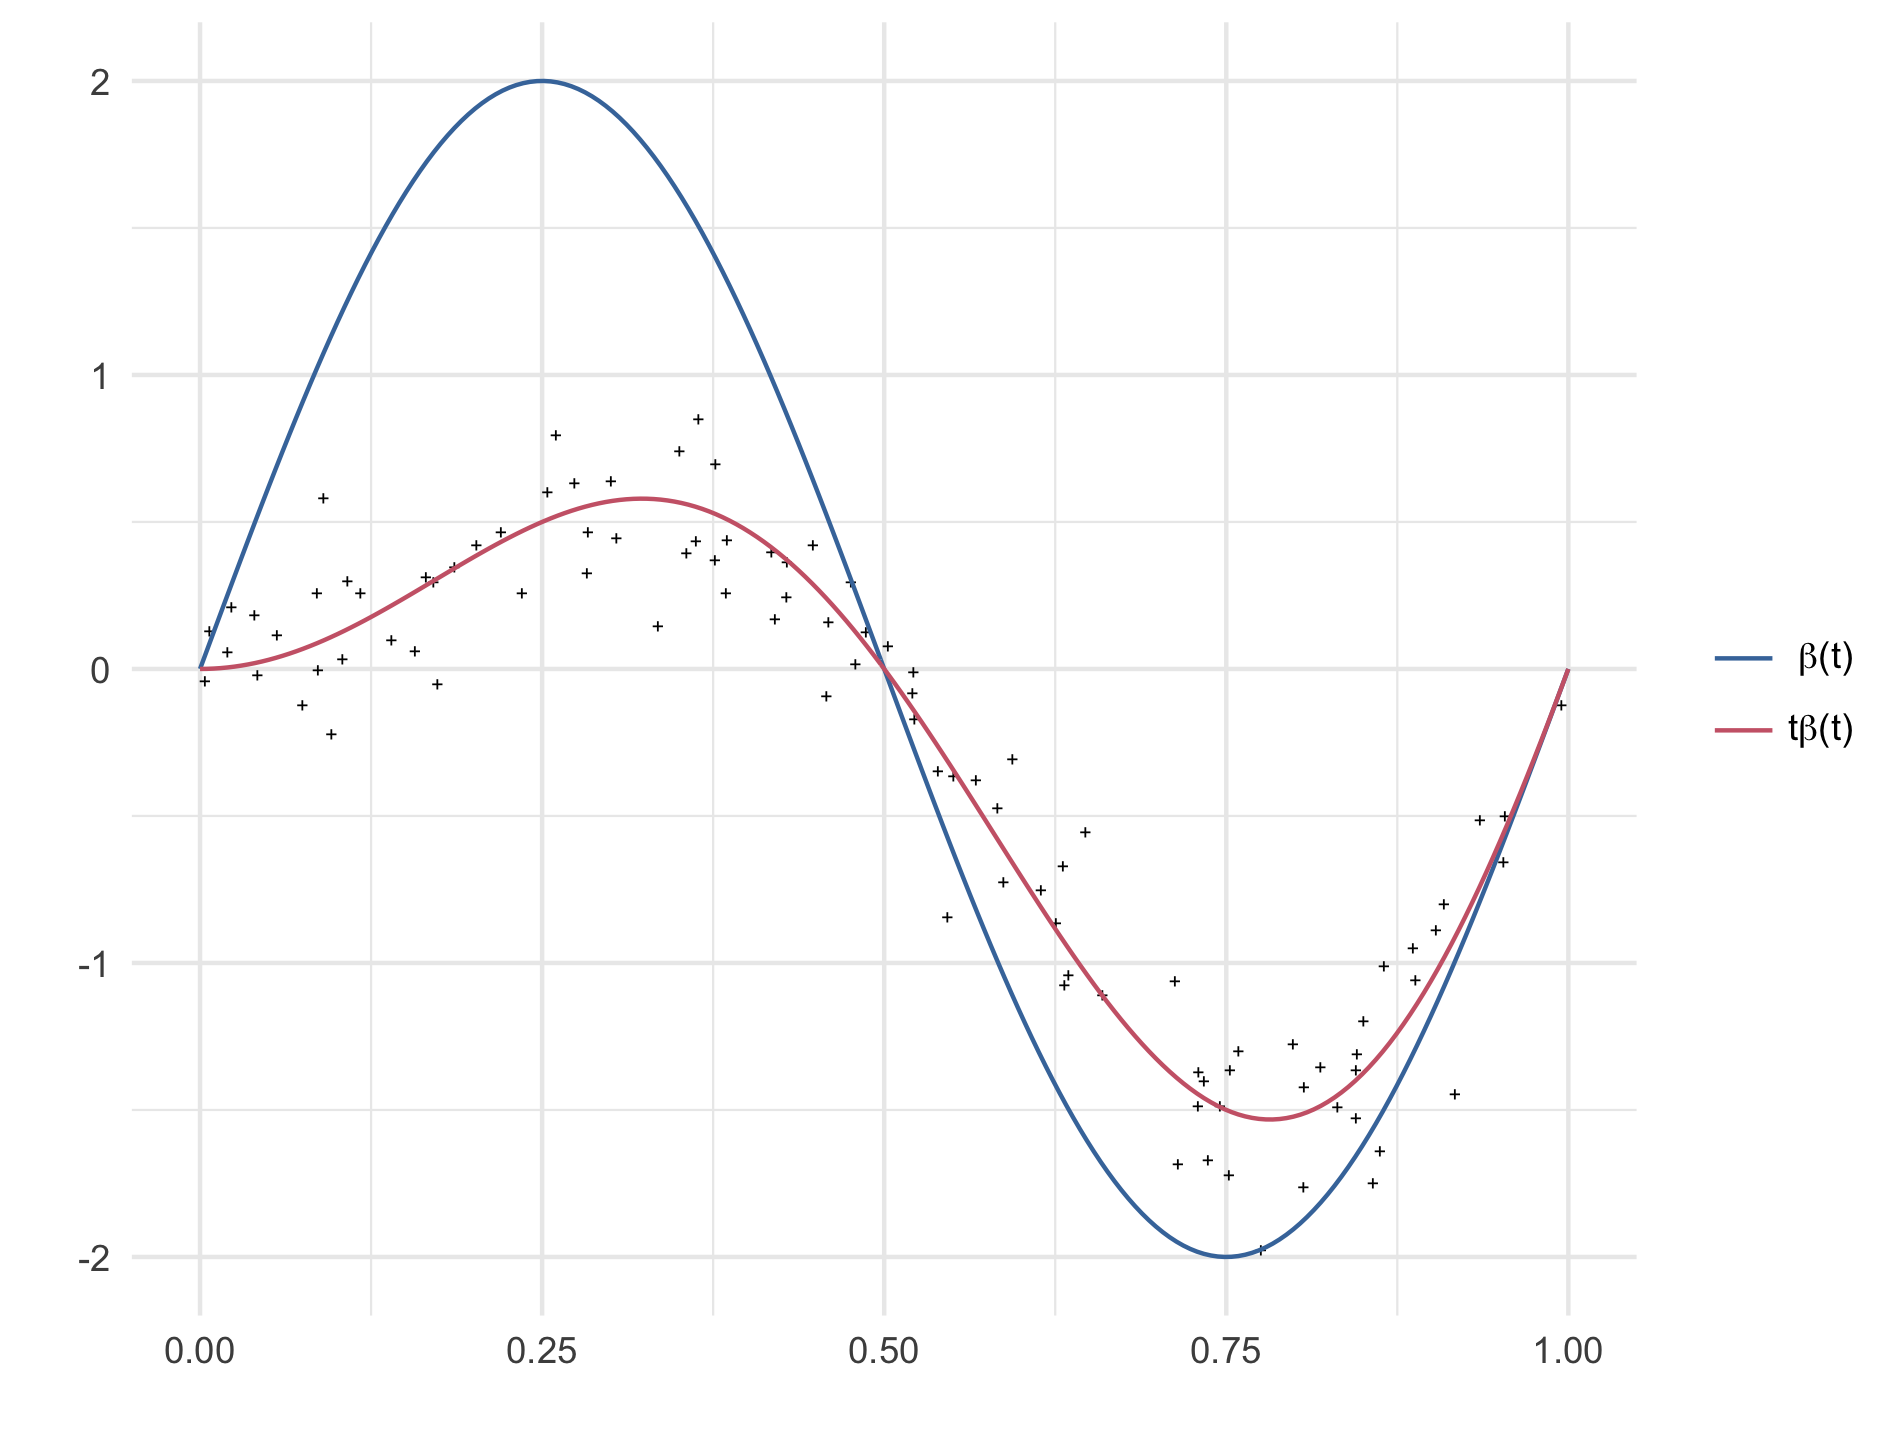
\includegraphics[scale=0.25]{PS_VCM_section_figure_1.png}
\caption{\textit{100 simulated data points where} $y\left(t\right) = t \beta\left( t \right) + 0.2\epsilon\left(t\right)$ \textit{where} $\epsilon$ \textit{is a white noise process with unit variance, and} $\beta\left(t\right) = 2\sin\left(2\pi t\right)$.}
\label{fig:PS_VCM_section_figure_1}
\end{figure}

\begin{figure}[H]
\begin{subfigure}{.5\textwidth}
  \centering
   \graphicspath{{img/}}
  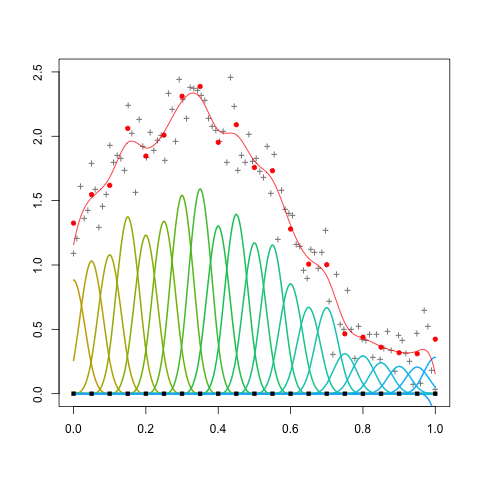
\includegraphics[scale=0.5]{pspline_pord2_xsmall_lambda.png}
  \label{fig:pspline_small_lambda}
\end{subfigure}
\begin{subfigure}{.5\textwidth}
  \centering
   \graphicspath{{img/}}
  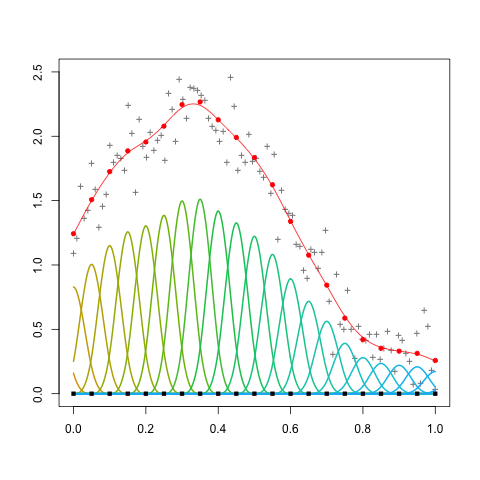
\includegraphics[scale=0.5]{pspline_pord2_small_lambda.png}
  \label{fig:pspline_small_lambda}
\end{subfigure}
\begin{subfigure}{.5\textwidth}
  \centering
   \graphicspath{{img/}}
  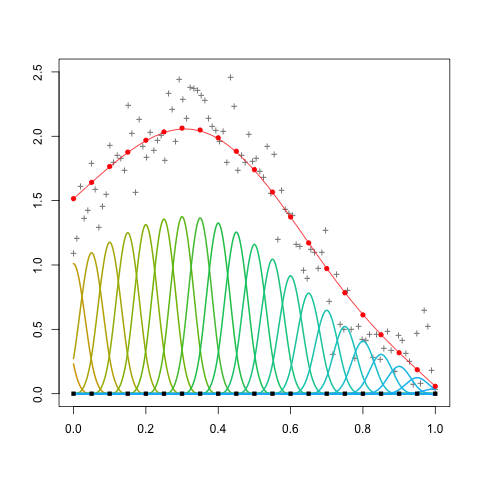
\includegraphics[scale=0.5]{pspline_pord2_medium_lambda.png}
  \label{fig:pspline_small_lambda}
\end{subfigure}
\begin{subfigure}{.5\textwidth}
  \centering
   \graphicspath{{img/}}
  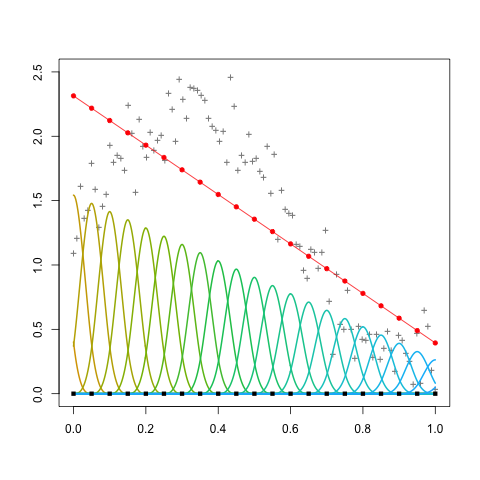
\includegraphics[scale=0.5]{pspline_pord2_large_lambda.png}
  \label{fig:pspline_small_lambda}
\end{subfigure}
\caption{\textit{Illustration of the impact of the second order difference penalty. The number of B-splines used is the same in each plot, with the value of the penalty parameter increasing from left to right and top to bottom across each plot. The fitted curve in the upper left plot is the most ``wiggly'' of any of the fits, as the penalty plays the weakest roll in the fitted coefficients there. The red circles are the values of each of the B-spline coefficients; as the penalty increases, they form as smoother sequence as we move across the four plots, which results in a smoother fitted function. As the penalty parameter approaches infinity, the fit approaches a linear function as shown in the bottom right plot.}}
\label{fig:second_ord_PS_pen_SML_lambda}
\end{figure}

The number of B-splines can be much larger than the number of observations because penalty ensures that the fitting procedure well-conditioned. One could literally use a thousand splines to fit ten observations without problems. Figure~\ref{fig:overcomplete_basis_pspline} illustrates this utility of the penalty for simulated data. There are $m=10$ observations and $40 + 3$ cubic B-splines. This property of P-splines cannot be overly appreciated, as it allows us to completely circumvent the nontrivial task of the optimal selection of knot placement. But one simply cannot have too many B-splines. Unless computational constraints are of concern, which is possible with large models, it is prudent to use even more. Figure~\ref{fig:PS_penalty_section_figure_3} shows how the fitted function changes as the tuning parameter $\lambda$ is varied in the presence of sparsely sampled data. 

\begin{figure}[H]   \label{fig:overcomplete_basis_pspline}
  \centering
   \graphicspath{{img/}}
  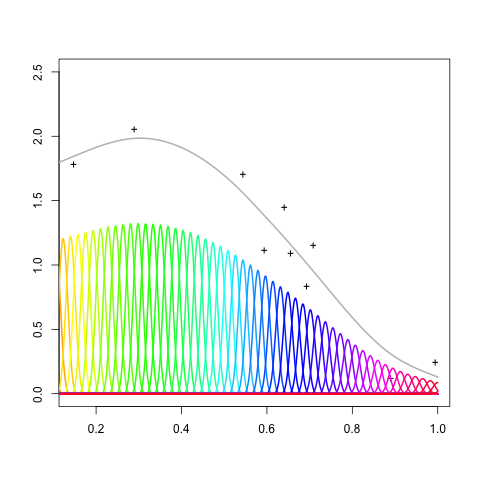
\includegraphics[scale=0.75]{pspline_10obs_60_basis_functions.png}
  \caption{P-spline smoothing of 10 observations using 60 B-spline basis functions.}
\end{figure}

\begin{figure}[H] \label{fig:PS_penalty_section_figure_3}
\centering
 \graphicspath{{img/}}
  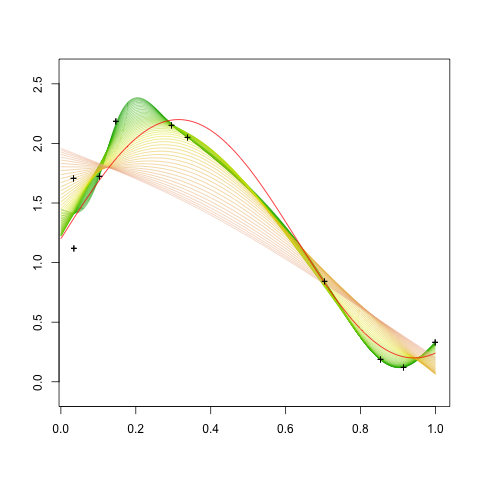
\includegraphics[width=4in, height=4in]{PS_penalty_section_figure_3.png}

  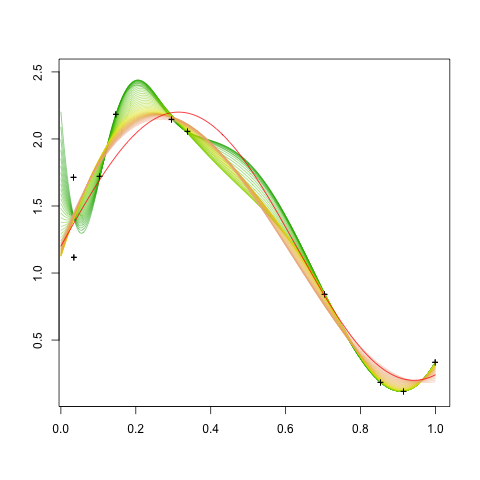
\includegraphics[width=4in, height=4in]{PS_penalty_section_figure_4.png}
 \caption{Fitted mean curves using a second (top) and third (bottom) order difference penalty for simulated data, sparsely sampled along the indexing variable: $y\left(t\right) = 1.2 + \sin\left(5t\right) + 0.2\epsilon_t$, where $\epsilon_t \stackrel{i.i.d.}{\sim}\textup{N}\left(0,1\right)$. A total of 10 data points were fit using a basis of 60 B-splines of degree $k=3$.}
\end{figure}

%%==============================================================================================================================================
%%==============================================================================================================================================
%%==============================================================================================================================================
%%==============================================================================================================================================
%%==============================================================================================================================================
%%%==============================================================================================================================================
%\subsection{Properties of P-splines}
%% \subfile{chapter-3-subfiles/chapter-3-properties-of-psplines}
%
%P-splines exhibit a number of advantageous properties, many of which are due to the inherited properties of the B-spline basis functions.
%
%\begin{enumerate} \label{eq:PS_properties}
%\item \begin{description}\item[Boundary effects]
% P-splines show no boundary effects, as many types of kernel smoothers do. By this, we mean the spreading of a fitted curve or density outside of the (physical) domain of the data, generally accompanied by bending toward zero.
%\end{description}
%\item \begin{description}\item[P-splines fit polynomial data exactly.] 
%P-splines can fit polynomial data exactly. Given data $\left(t_i,y_i\right)$, if the $y_i$ are a polynomial in $t$ of degree $k$, then B-splines of degree $k$ or higher will fit the data exactly. 
%\begin{proof}
%This statement is equivalent to the claim that given $\xi = \left\{ \xi_i \right\}$, $i=1,\dots,l+1$, and $g$ such that $y\left(t\right) = g\left(t\right)$, we can find an $f \in \PP_{k,\xi} \bigcap \mathscr{C}^{\left(k-2\right)}$ which agrees with $g$ at the points $\tau_1 < \dots < \tau_n$  with $\tau_i \in \left[\xi_1,\xi_{l+1}\right]$ for all $i$, where
%\[
%n=k+l-1
%\]
%The solution, $f$ is constructed as follows: generate the knot sequence $t = \left\{t_i\right\}$ as per the recipe in Theorem~\ref{curryschoenbergthm}:
%\begin{align*}
%t_1 &= t_2 = \dots = t_k = \xi_1 & \\
%t_{k+i} &= \xi_{i+1}, & i=1,\dots,l-1\\
%t_{n+1} &= t_{n+2} = \dots = t_{n+k} = \xi_{l+1} & 
%\end{align*}
%
%Let $\left\{ B_{ik} \right\}$, $i=1,\dots,n$ be the corresponding sequence of B-splines of order $k$, which are a basis for $\PP_{k,\xi} \bigcap \mathscr{C}^{\left(k-2\right)}$ by Theorem~\ref{curryschoenbergthm}. Here, $\PP_{k,\xi} \bigcap \mathscr{C}^{\left(k-2\right)}$ denotes the space of pp functions with breakpoints $\xi$ having two continuous (global) derivatives. Then, \cite{schoenberg1953polya} have shown that there exists exactly one $f \in \PP_{k,\xi} \bigcap \mathscr{C}^{\left(k-2\right)}$ agreeing with $g$ at $\tau_1,\dots, \tau_n$ if and only if 
%\[
%B_{ik}\left(\tau_i\right) \ne 0, \qquad \qquad i=1,\dots,n.
%\]
%This $f$ has a unique expansion of the form
%\[
%f = \sum_{i=1}^n a_i B_{ik}
%\] 
%for coefficients $a_i,\dots, a_n$, which are the solution to the linear system
%\[
%\sum_{j=1}^n a_jB_{jk}\left(\tau_i\right) = g\left(\tau_i\right), \qquad \qquad i=1,\dots,n.
%\]
%This system has a banded matrix of coefficients since $B_{jk}\left(\tau_i\right) \ne 0$ if and only if $\tau_i \in \left[t_j,t_{j+k}\right]$. So if $B_{jk}\left(\tau_i\right) \ne 0$ and thus $\tau_i \in \left(t_j,t_{j+k}\right)$, then there are at most $k$ of the $j$ indices such that $B_{jk}\left(\tau_i\right)$ is nonzero. And further, each of these indices $j$ must be such that 
%\[
%\left(t_i,t_{i+k}\right) \bigcap \left(t_j,t_{j+k}\right) \ne \emptyset,
%\]
%or such that $\vert i-j \vert < k$. At worst, the system corresponds to a banded matrix with $k-1$ lower and $k-1$ upper diagonals. 
%\end{proof}
%The same is true for P-splines if the order of the penalty is $k+1$ or higher, irrespective of the value of $\lambda$. Consider imposing a first-order difference penalty and a fit to data $y$ that is constant - a polynomial of degree 0. Since 
%\[
%\sum_{j=1}^n \hat{\alpha}_j B_j\left( x_i \right) = c, 
%\]
%\noindent
%we have that
%\[
%\sum_{j=1}^n \hat{\alpha}_j B^\prime_j\left( x \right) = 0, 
%\]
%\noindent
%for all $x$. From the relationship between differences and derivatives in \ref{eq:more_BS_properties} \ref{eq:BS_deriv_property}, 
%
%\[
%0 = \sum_{j=1}^n B^\prime_{j,k}\left(x\right) = \sum_{j=1}^n \Delta\alpha_{j+1} B_{j,k-1}\left( x \right), 
%\]
%\noindent
%so that we must have $\Delta \alpha_j = 0$ for all $j$, and 
%\[
%\sum_{j=2}^n \Delta \alpha_j = 0.
%\]
%
%This shows that the penalty has no impact on the basis coefficients, and the resulting fit is identical to that when using unpenalized B-splines. Using induction, one can show that this is also true when the relationship between $x$ and $y$ is linear and a second order difference penalty is used, and for any values of the polynomial order and order of the difference penalty.\end{description}
%\item \begin{description}\item[Null models under difference penalties] \label{eq:PS_property_3}
%The limiting P-spline fit approaches a polynomial under strongly enforced smoothing. As $\lambda \rightarrow \infty$, under a difference penalty of order $d$, the fitted function will approach a polynomial of degree $d-1$ as long as the degree of the B-splines is greater than or equal to $k$. To see this, we again need to use the relationship between the differenced coefficient sequence and the derivative of a B-spline as described in \ref{eq:more_BS_properties} \ref{eq:BS_deriv_property}. Consider using the second-order difference penalty; when $\lambda$ is large, the penalty dominates the P-spline objective function defined in \ref{eq:S_pen_varying_intercept_model}, so that the minimizer $\alpha$ must be such that $\sum_{j=3}^n\left(\Delta^2\alpha_j\right)^2$ is close to zero. Consequently, each of the individual second differences must also be nearly zero, and thus the second derivative of the fitted function must be close to zero over the entire domain.
%\end{description}
%\item \begin{description}\item[The limiting behaviour of $H_\lambda$] The trace of the hat matrix, 
%\[
%H_\lambda = B\left(B^TB + \lambda D_k^TD_k\right)^{-1}B^Ty
%\] 
%(or for $H$ defined for the addition of a varying slope component as in \ref{eq:simplest_VC_model_hat_matrix}) approaches $k$, the order of the differencing operator, as $\lambda$ increases. We index $H$ with the smoothing parameter to indicate that the elements of $H$ are a function of $\lambda$. Let
%\begin{equation}
%Q_B = B^T B \qquad \mbox{and} \qquad Q_\lambda = \lambda D^T D.
%\end{equation}
%Then using properties of the matrix trace, we can write
%\begin{align}
%\begin{split}
%\mbox{tr}\left(H_\lambda \right) &= \mbox{tr}\bigg[ \left(Q_B + Q_\lambda \right)^{-1}Q_B \bigg]\\
%&=\mbox{tr}\bigg[ Q_B^{1/2}\left(Q_B + Q_\lambda \right)^{-1}Q_B^{1/2} \bigg] \\
%&=\mbox{tr}\bigg[\left(I + Q_B^{-{1/2}}Q_\lambda Q_B^{-{1/2}} \right)^{-1} \bigg]
%\end{split}
%\end{align}
%Define $L \equiv Q_B^{-{1/2}}Q_\lambda Q_B^{-{1/2}}$. Then
%\begin{equation}
%\mbox{tr}\left(H_\lambda \right) = \mbox{tr}\bigg[\left(I + \lambda L \right)^{-1} \bigg] = \sum_{j=1}^n \frac{1}{1 + \lambda \gamma_j}
%\end{equation}
% where $\gamma_j$, $j=1,\dots,n$ are the eigenvalues of $L$. $Q_\lambda$ has exactly $k$ eigenvalues equal to zero, hence $L$ has $k$ zero eigenvalues. For large $\lambda$, only the $k$ terms with $\gamma_j=0$ contribute to the sum which gives the trace of $H$, so that
% \[
%\lim_{\lambda \rightarrow \infty  } \mbox{tr}\left(H\right) = k.
% \]
%\end{description}
%\end{enumerate}
%
%The previous derivations hold regardless of whether we are fitting the varying intercept-only model, with $\mu\left( t\right) = \beta_0\left(t\right)$ or accommodating a varying slope for a regressor by specifying $\mu\left( t\right) = \beta_0\left(t\right) + \beta_1\left(t\right)x\left(t\right)$. The inspection of the hat matrix $H$ is a prelude to the following section, where we will discuss how to use the properties of $H$ to tune the smoothing parameter for optimal model selection. We will later show that extension of these results can be extended in a rather straightforward manner to the case that is of our particular interest: when the smooth slope function is a two-dimensional surface rather than a curve.


\begin{figure}[h]
\centering
 \graphicspath{{img/}}
  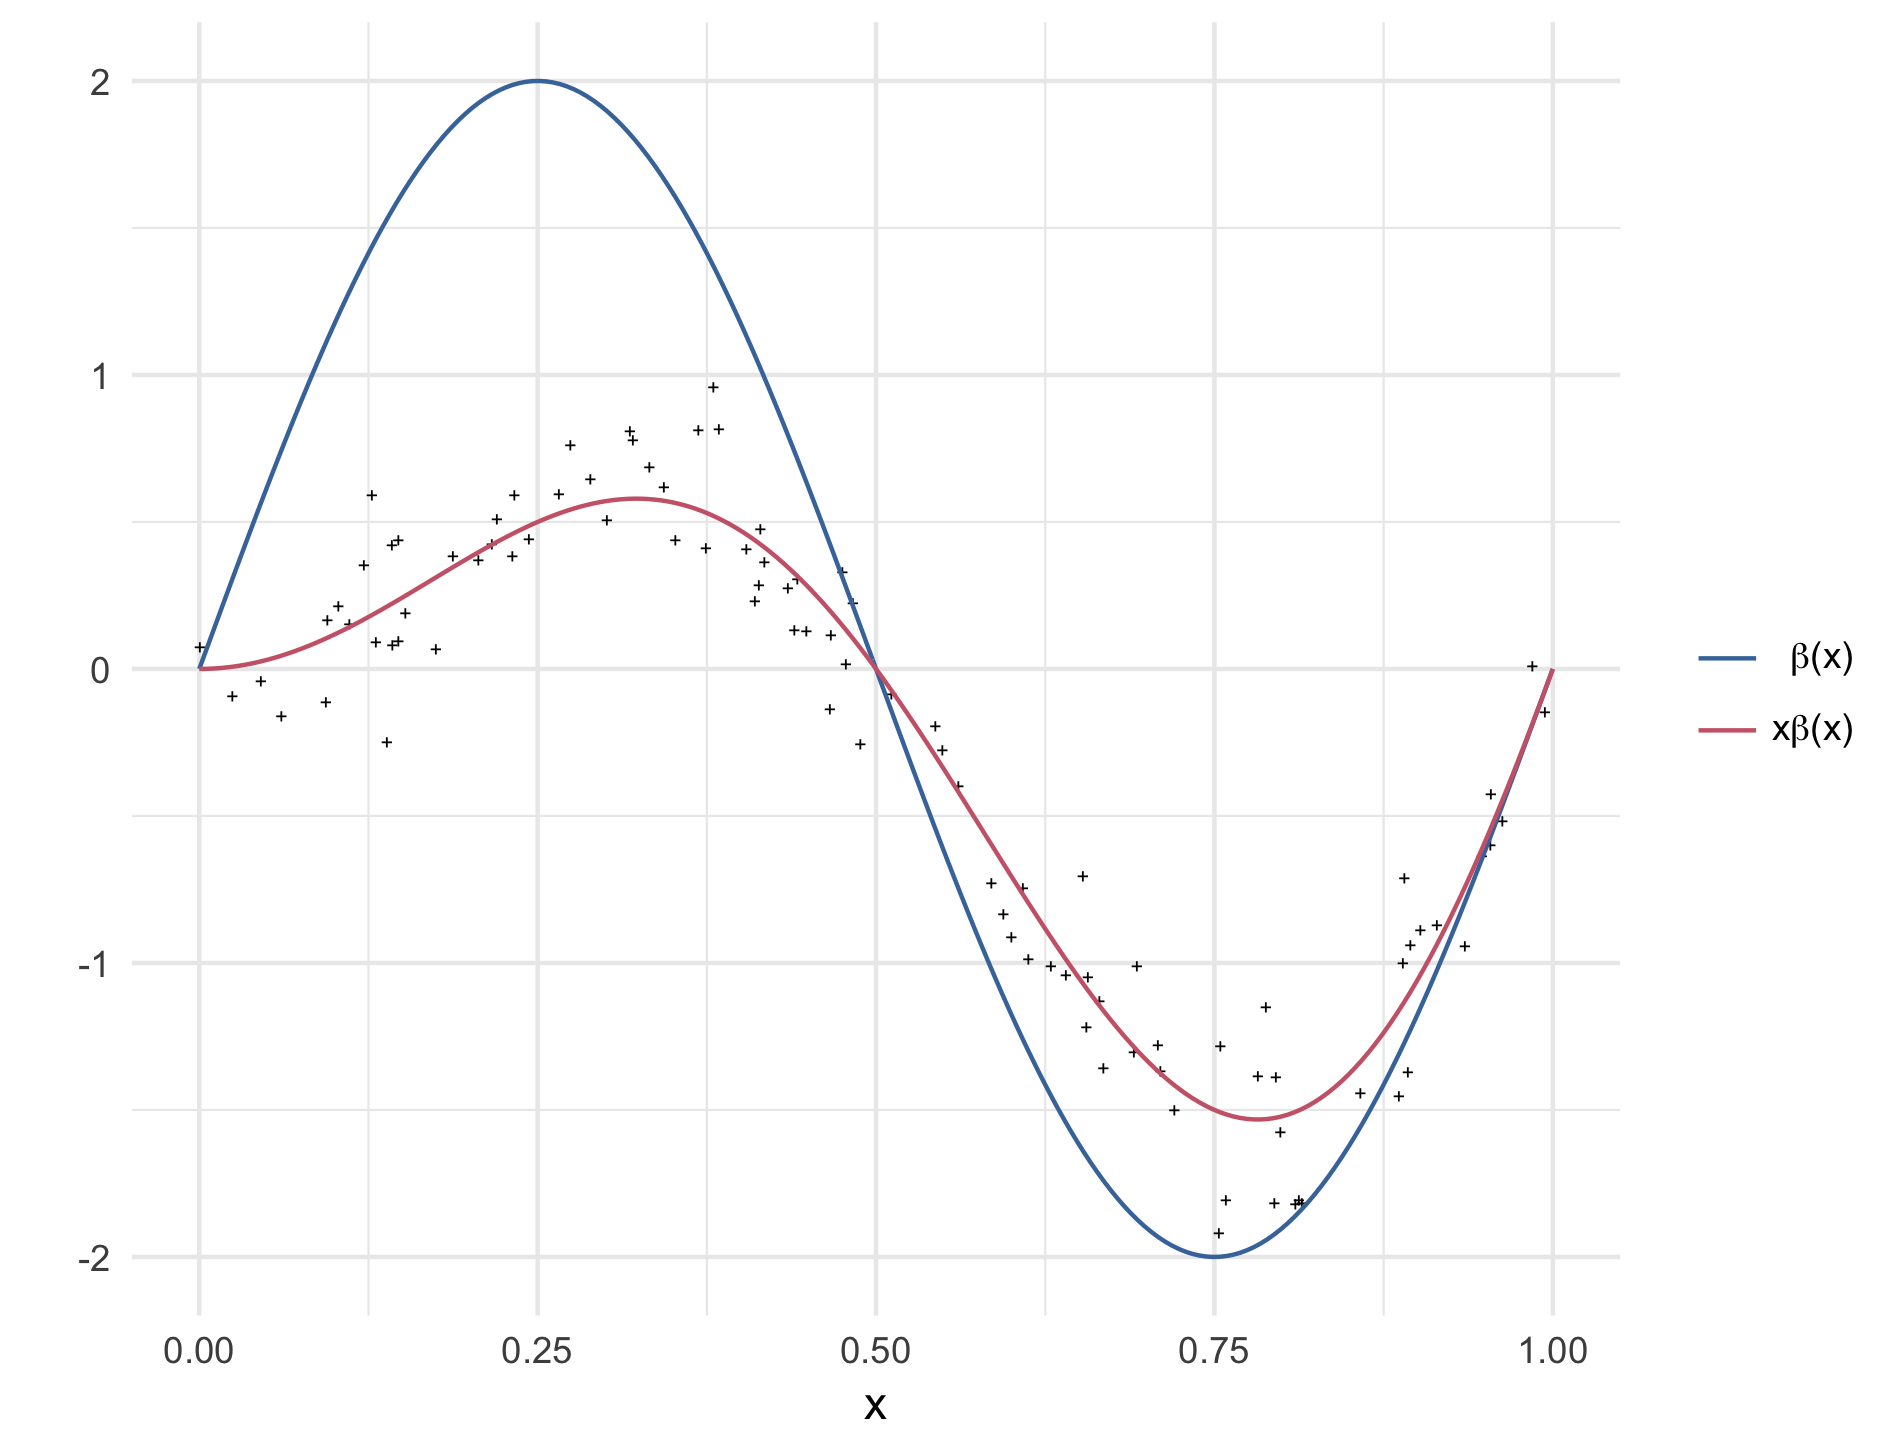
\includegraphics[width=4in, height=4in]{PS_penalty_section_figure_5.png}
 %\caption{Tensor product of two cubic B-splines}
\end{figure}
%%==============================================================================================================================================
%%==============================================================================================================================================
%%==============================================================================================================================================
%%==============================================================================================================================================
%%==============================================================================================================================================
%%==============================================================================================================================================

%%==============================================================================================================================================
%%==============================================================================================================================================
%%==============================================================================================================================================
%%==============================================================================================================================================
%%==============================================================================================================================================
%%==============================================================================================================================================
\subsection{The reguarlized MLE for $\phi$ via tensor product P-splines}
% \subfile{chapter-3-subfiles/chapter-3-tensor-product-pspline-MLE}
To extend the P-spline framework to allow estimation of a bivariate function, $\phi$, we simply need to equip the $l$ and $m$ axes each with a B-spline basis. A basis for the varying coefficient function is constructed taking the tensor product of the two marginal bases. Let 
\[
B_{1}\left(l\right),\dots, B_{K}\left(l\right)  \mbox{ and } B_{1}\left(m\right),\dots, B_{L}\left(m\right)
\]
denote the B-spline bases for $l$ and $m$, each having a set of equally spaced knots along their respective domain. It is worth noting that while we have chosen not to distinguish between $\left\{ B_k \right\}$ and $\left\{ {B}_l \right\}$ for the sake of brevity, one is free to specify a different basis for each dimension either by using different order B-spline or, of course, using different numbers of knots, and hence entirely different knot sequences since P-splines rely on bases with equally spaced knots. The tensor product basis functions
\begin{equation*}
T_{jk}\left(l,m\right) = B_j\left(l\right){B}_k\left(m\right)
\end{equation*}
\noindent
carve the $l$-$m$ domain into rectangles.  Figure~\ref{fig:sparse_bicubic_BS_basis} shows a thinned tensor product basis $\left\{ T_{kl} \right\}$; a portion of the basis was omitted to eliminate overlapping of the basis functions so that the reader can identify individual tensor products. Each ``hill'' in Figure~\ref{fig:sparse_bicubic_BS_basis} is associated with an unknown coefficient $\theta_{ij}$ which determines the height of the hill. For a given knot grid, we can approximate a surface by

\begin{equation} \label{eq:varying-coefficient-tensor-product-expansion}
\phi\left(l,m\right) = \sum_{i=1}^K \sum_{j=1}^L \theta_{ij} B_{i}\left(l\right) B_{j}\left(m\right), 
\end{equation}
\noindent
and the function evaluated at the observed $\left(l_{ijk}, m_{ijk}\right)$ may be written 
\begin{equation*} 
\vphistar = B_m \Theta B_l^\prime
\end{equation*}
\noindent 
where $\Theta$ denotes the $K \times L$ matrix of tensor product coefficients, with elements $\theta_{ij}$.

\begin{figure}[H]
\centering
 \graphicspath{{img/}}
  \includegraphics[width=4in, height=4in]{bicubic_basis_function.png}
 
\includegraphics[width=4in, height=4in]{bicubic_bspline_contour.png}
\caption{Tensor product of two cubic B-splines}
\label{fig:bicubic_BS}
\end{figure}

\begin{figure}[H]
  \centering
  \graphicspath{{img/}}
  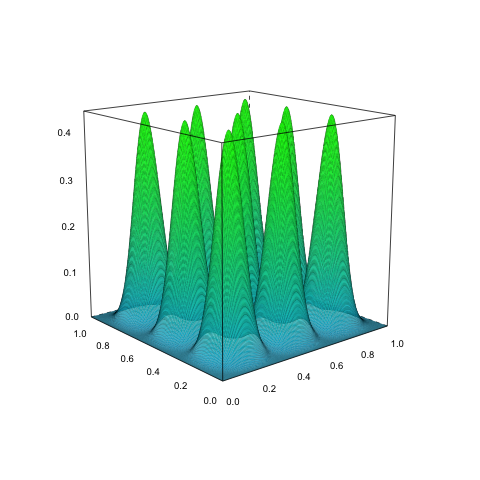
\includegraphics[width=5in,height=5in]{sparse_bicubic_basis.png}
  \caption{A subset of a full bivariate basis of cubic B-splines}\label{fig:sparse_bicubic_BS_basis}
\end{figure}

\subsection{Regularization with difference penalties} \label{subsection:univariate-psplines}

The minimizer of \ref{eq:loglikelihood} honors the fidelity to the data, so to balance the complexity of the fitted function with the goodness of fit to the data, we can append a penalty to the negative log likelihood to control the fitted function. By using rich B-spline bases for $l$ and $m$ alongside discrete difference penalties on the spline coefficients, we can achieve as much smoothness of the fitted function in both the $l$ and $m$ dimensions as desired. \cite{o1986statistical} was the first to propose using a rich B-spline basis and using a penalty to restrict the flexibility of the fitted curve, like \cite{wahba1990spline} applying a penalty to the second derivative of the fitted curve:
\[
J = \int_0^1 \left[ f^{\prime \prime}\left(l\right)\right]^2\;dx.
\]

For a B-spline of the form
\[
f\left(x\right) = \sum\limits_{j=1}^n \theta_i B_j\left(x\right),
\]
one can derive a banded matrix $P$ using the properties of B-splines such that 
 \[
 J = \theta^\prime P \theta
 \] 
 \noindent
 where $\theta = \left(\theta_1,\dots, \theta_n\right)$. The $i$-$j^{th}$ element of $P$ is given by
 \[
 p_{ij} = \int_0^1 B_i^{\prime \prime} \left( x \right)B_j^{\prime \prime} \left( x \right)\;dx.
 \]

%As discussed in Section 2, we can define an entire class of functional autoregressive models using only the $l$ direction, and additionally, as discussed in Section 3, there is a natural expectation about the functional form of the autoregressive coefficient function (and hence covariance) as a function of $l$. The use of smoothing splines to estimate $\phi$ outlined in Section~\ref{} yields smooth null models, but smoothness of the elements of the Cholesky factor alone may not lead to desirable structure in the inverse covariance matrix.  

%
%These approaches implicitly adopt different notions of sparsity. Like \cite{huang2006covariance} and \cite{levina2008sparse}, our aim is to regularize the inverse of the covariance matrix through the Cholesky factor. Expressing the varying coefficient function using a tensor product basis expansion builds the foundation for a flexible estimation framework within which employing multiple notions of smoothness is simple and straightforward. 
%

In some applications, it is useful to work with third and fourth order differences, since for large values of $\lambda$, the fitted curve approaches a parametric polynomial model. This may be of particular interest in the context of estimating the elements of the Cholesky factor, as many have proposed simple parametric functions of lag only for $\phi$, such as low order polynomials. See \cite{pourahmadi1999joint}. However, with the use of higher order derivatives, the computation of $P$ is nontrivial and becomes very tedious. \cite{eilers1996flexible} were the first to propose P-splines, or \emph{penalized B-splines}, as an approach to nonparametric regression. P-splines circumvent complexity associated with constructing such penalty matrices by omitting derivatives and integrals altogether, replacing them with finite differences and sums. 

Instead, flexibility of the fitted function is controlled by using a discrete penalty matrix based on finite difference formulas. Smoothness of the fitted function is achieved by first using a rich B-spline basis with equally spaced knots to purposefully overfit the smooth coefficient vectors; this eliminates the difficulty of choosing the optimal set of knots. Then by attaching a difference penalty to the goodness of fit measure, one may prevent overfitting and make a potentially ill-conditioned fitting procedure a well-conditioned one. The finite difference penalty is simple to compute and can be handled mechanically for any order of the differences. Since it is easily introduced into regression equations, it is feasible to evaluate the impact of different orders of the differences on the fitted model.  Using the properties of B-splines, it is straightforward to show that the difference penalty of order $d$ is a good discrete approximation to the integrated square of the $d^{th}$ derivative, so little is lost by replacing the derivative-based penalty with

\begin{equation} \label{eq:bspline-difference-penalty}
J_d\left( f \right) = \sum_{j=d}^n \left(\Delta^d \theta_j\right)^2
\end{equation} 
\noindent
where $\theta = \left( \theta_1,\dots,\theta_n \right)$. Let $D_d$ denote the matrix difference operator: $D_d\theta = \Delta^d \theta$, where

 \begin{align*}
 \Delta \theta_j &= \theta_j - \theta_{j-1}, \quad  \Delta^2 \theta_j = \Delta\left(\Delta \theta_j\right) = \theta_j - 2\theta_{j-1} + \theta_{j-2}
 \end{align*}
\noindent 
In general,
\begin{equation*}
\Delta^d \theta_j = \Delta\left(\Delta^{d-1} \theta_j \right).
\end{equation*} 
\noindent
Then, \ref{eq:bspline-difference-penalty} can be written in terms of the squared norm of the difference operator applied to the vector of B-spline coefficients:
\begin{align} 
\begin{split} \label{eq:bspline-difference-penalty-vector-form}
J_d\left( f \right) &= \vert \vert D_d\theta \vert \vert^2 \\
&= \theta^\prime P_d \theta
\end{split}
\end{align}
\noindent
where $P_d = D_d^\prime D_d$.  To examine the connection between the second-derivative penalty to the penalty on second-order differences of the B-spline coefficients, we only need to employ straightforward calculus and exploit the recursive property of the B-spline basis functions:

\begin{equation*} 
\int_0^1 \left[ f^{\prime \prime}\left(x\right)\right]^2\;dx = \int_{0}^{1} \left\{ \sum\limits_{j=1}^n  \theta_j B_{j,3}^{\prime \prime} \left(l\right) \right\}^2\; dl.
\end{equation*}
\noindent
The derivative properties of B-splines permits this to be written as 
\begin{equation*} \label{eq:second-derivative-bspline-penalty}
\int_0^1 \left[ f^{\prime \prime}\left(x\right)\right]^2\;dx =  \int_{0}^{1}  \bigg[ \sum\limits_{j=1}^n \sum\limits_{k=1}^n \Delta^2 \theta_j \Delta^2 \theta_k B_{j,1}\left(l\right)B_{k,1}\left(l\right)\bigg]\; dl  . 
\end{equation*}
\noindent
Most of the cross products of $B_{j,1}\left(x\right)$ and $B_{k,1}\left( x \right)$ vanish since B-splines of degree 1 only overlap when $j$ is $k-1$, $k$, or $k+1$. Thus, we have that
\begin{align}
\begin{split}
\int_0^1 \left[ f^{\prime \prime}\left(x\right)\right]^2\;dx  = {} &  \int_0^1 \bigg[ \left\{ \sum\limits_{j=1}^n   \Delta^2 \theta_j  B_j\left(l,1\right)  \right\}^2  + 2 \sum_{j}\Delta^2 \theta_j\Delta^2 \theta_{j-1}B_j\left(l,1\right)B_{j-1}\left(l,1\right) \bigg]\; dl \\ 
= {} & \sum \limits_{j=1}^n  \left( \Delta^2\theta_j \right)^2 \int_0^1 B_j^2\left(l,1\right)\;dl \\
   &{} \;\;\;\;\;\;\;\;\;\;\;\;\;\;\;\;\;\; + 2 \sum\limits_{j=1}^n \Delta^2 \theta_j\Delta^2 \theta_{j-1} \int_0^1 B_j\left(l,1\right)B_{j-1}\left(l,1\right)\;dl 
\end{split}
\end{align}
\noindent
which can be written as
\begin{equation} \label{eq:derivative-penalty-difference-penalty-connection}
\int_0^1 \left[ f^{\prime \prime}\left(x\right)\right]^2\;dx  = c_1 \sum\limits_{j=2}^n \left( \Delta^2 \theta_j\right)^2 + c_2 \sum\limits_{j=3}^n \Delta^2 \theta_j\Delta^2 \theta_{j-1}
\end{equation}
\noindent
Given a set of equidistant knots, the constants $c_1$ and $c_2$ are given by
\begin{equation}
\begin{split}
c_1 & =   \int_0^1 B_{j,1}^2\left(x\right) dx\\
c_2 & = \int_0^1 B_{j,1}\left(x\right)B_{j-1,1}\left(x\right) dx.
\end{split}
\end{equation}

This gives us that the traditional smoothness penalty on the squared second derivative can be written as a linear combination of a penalty on the second-order differences of the B-spline coefficients \ref{eq:bspline-difference-penalty} and the sum of the cross products of neighboring second differences. The second term in \ref{eq:derivative-penalty-difference-penalty-connection} leads to a complex objective function when minimizing the penalized likelihood, where seven adjacent spline coefficients occur, as opposed to five if only the first term in \ref{eq:derivative-penalty-difference-penalty-connection} is used in the penalty. The added complexity is a consequence of overlapping B-splines, which quickly increases when using higher order differences and higher order B-splines. We can seamlessly augment the likelihood with the difference penalty to achieve smooth fitted functions without the complexity posed by the derivative-based penalty.
%citet{chen2011efficient}, citet{pourahmadi1999joint}, and citet{pourahmadi2002dynamic} have elicited parametric models for the generalized autoregressive coefficients, letting the GARPs depend only on the distance between two time points.

A smoother sequence of coefficients leads to a smoother curve, as illustrated in Figure~\ref{fig:second_ord_PS_pen_SML_lambda}.  The relationship between P-spline curves and their coefficients is easily characterized if we consider the coefficients as the skeleton of the function, and draping the B-splines over them puts the flesh on the bones. As long as the coefficient sequence is smooth, the number of basis functions (and coefficients) is unimportant since the penalty ensures the smoothness of the skeleton and that the fitting procedure is well-conditioned. Figure~\ref{fig:overcomplete_basis_pspline} illustrates this utility of the penalty for simulated data; there are $m=10$ observations and $60$ cubic B-splines. This property of P-splines cannot be overly appreciated because it frees us from the concern of choosing the optimal set of knots. Unless computational constraints are of concern, which is possible with large models, it is prudent to use even more B-splines. Figure~\ref{fig:PS_penalty_section_figure_2} shows how the fitted function changes as the tuning parameter varies when the data are sparsely sampled. P-splines enjoy a number of additional advantageous properties, many of which are inherited from the attractive properties of B-splines. See \cite{eilers1996flexible}  for a detailed presentation. 

\begin{figure}[H] \label{fig:PS-smoothing-figure-1}
\begin{subfigure}{.5\textwidth}
  \centering
   \graphicspath{{img/}}
  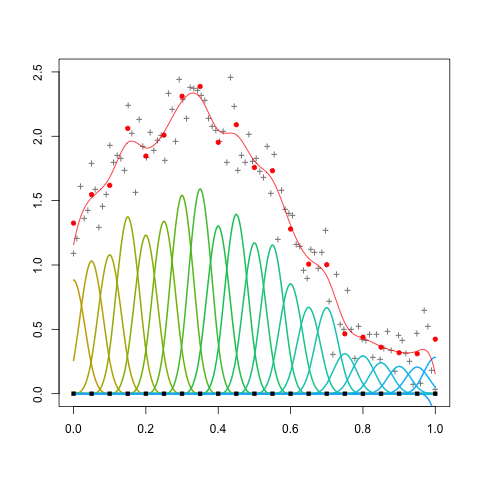
\includegraphics[scale=0.5]{pspline_pord2_xsmall_lambda.png}
  \label{fig:pspline_small_lambda}
\end{subfigure}
\begin{subfigure}{.5\textwidth}
  \centering
   \graphicspath{{img/}}
  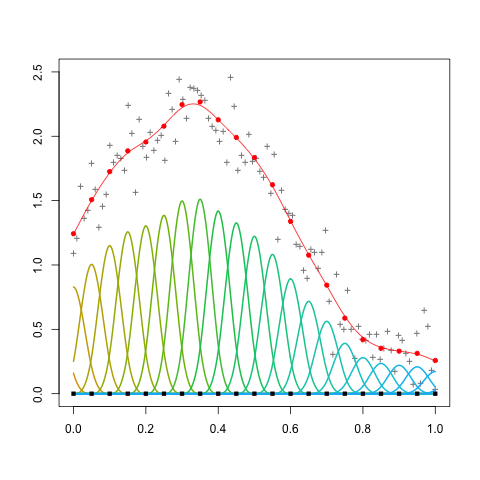
\includegraphics[scale=0.5]{pspline_pord2_small_lambda.png}
  \label{fig:pspline_small_lambda}
\end{subfigure}
\begin{subfigure}{.5\textwidth}
  \centering
   \graphicspath{{img/}}
  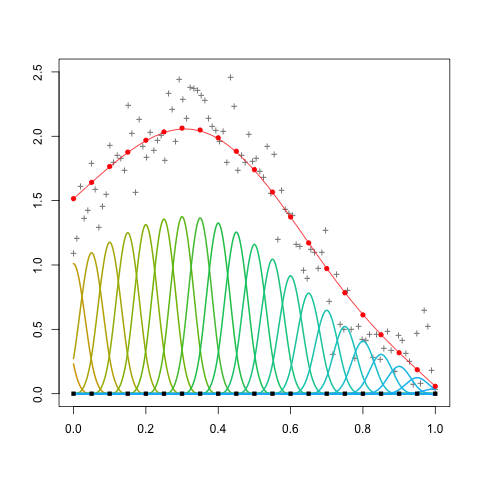
\includegraphics[scale=0.5]{pspline_pord2_medium_lambda.png}
  \label{fig:pspline_small_lambda}
\end{subfigure}
\begin{subfigure}{.5\textwidth}
  \centering
   \graphicspath{{img/}}
  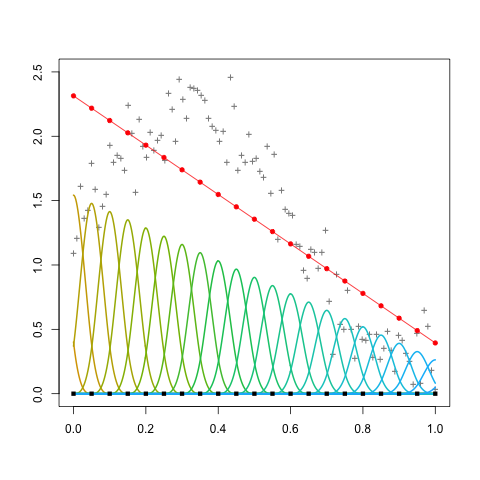
\includegraphics[scale=0.5]{pspline_pord2_large_lambda.png}
  \label{fig:pspline_small_lambda}
\end{subfigure}
\caption{\textit{Illustration of the impact of the second order difference penalty. The number of B-splines used is the same in each plot, with the value of the penalty parameter increasing from left to right and top to bottom across each plot. The fitted curve in the upper left plot is the most ``wiggly'' of any of the fits, as the penalty plays the weakest roll in the fitted coefficients there. The red circles are the values of each of the B-spline coefficients; as the penalty increases, they form as smoother sequence as we move across the four plots, which results in a smoother fitted function. As the penalty parameter approaches infinity, the fit approaches a linear function as shown in the bottom right plot.}}
\label{fig:second-ord-PS-pen-SML-lambda}
\end{figure}
%%==============================================================================================================================================
%%==============================================================================================================================================
%%==============================================================================================================================================
%%==============================================================================================================================================
%%==============================================================================================================================================
%%==============================================================================================================================================


%We employ maximum likelihood  for the estimation of  the varying coefficient function $\phi\left(t,s\right)$ and the innovation variance function $\sigma\left(t\right)$, though neither the derivation the form of model~\ref{eq:ARmodel} nor model~\ref{eq:MyModel} via the Cholesky decomposition rely on any assumptions about the distribution of $Y$. 
%
%For fixed $\left\{ \sigma_j^2 \right\}$, as a function of $\phi_{jk}$ the negative log-likelihood for a sample of $N$  i.i.d. observations $Y_1,Y_2,\dots,Y_N$ from a multivariate Gaussian distribution is proportional to the usual error sums of squares:
%
%\begin{equation}
%-2 L\left(y_1,\dots,y_N ,\phi \vert \vsigmasq \right) \propto \sum_{i=1}^N \sum_{j=2}^{m_i} \sigma\left({t_j}\right)^{-2} \left(y_{ij} - \sum_{k=1}^{j-1}\phi\left({t_{ij},t_{ik}}\right)y_{ik} \right)^2 \label{loglikelihood}
%\end{equation}
%\noindent
%where 
%\[
%y_i = \left( y_{i1}, y_{i2}, \dots, y_{i,m_i}\right), \quad i=1,\dots,N 
%\] 
%
%%% explain here that we omit y_{i1} from the likelihood here because in the first stage of estimation (for $\phi$), the first observation in each vector doesn't contribute to the likelihood
%\noindent
%denotes the vector of observations for subject $i$ with corresponding measurement times 
%\[
%t_{i1} < t_{i2} < \dots < t_{i,m_i}.
%\]
%The form of the likelihood of $y_1,\dots,y_N$ indicates that we allow both the number of measurements as well as the observation times to varying across subjects. The $\left\{t_{ij} \right\}$ need not be evenly-spaced within or across individuals. Denote the innovation variance function evaluated at the vector of observed time points by $\vsigmasq$, and similarly let $\vphistar$ denote the resulting vector when evaluating $\phi$ at the observed grid of time points, transformed to the $l$-$m$ axis. Estimation of the varying coefficient function and the innovation variance function may be accomplished in an iterative fashion:
%
%\fbox{\parbox{\textwidth}{\begin{enumerate}
%\item Fix $\vsigmasq = \vsigmasq_0$;
%\item find $\widehat{\vphistar} = \underset{\vphistar}{\arg\max} -2 L\left(y_1,\dots,y_N ,\vphistar \vert \vsigmasq_0 \right)$.
%\item Fix $\vphistar= \widehat{\vphistar}$;
%\item find $\widehat{\vsigmasq} = \underset{\vsigmasq}{\arg\max} -2 L\left(y_1,\dots,y_N , \vsigmasq \vert \widehat{\vphistar} \right)$.
%\item Iterate until convergence.
%\end{enumerate}}}
%
%\vspace{0.5cm}


% 
%\section{\emph{Penalized maximum likelihood estimation}}
%
%\begin{enumerate}
%\item Fix $\sigma_{ij}^2 = \sigma_{ij0}^2$, $i=1,\dots,N$ ,$j=1,\dots,M$.
%\item Find $\phi_0 = \underset{\phi}{arg \; min} -2L_\phi\left(\phi, y_1,\dots, y_N \right) + \lambda J\left( \phi \right)$
%\item Fix $\phi = \phi_{0}$.
%\item Find  $\sigma_{0}^2 = \underset{\sigma^2}{arg\; min} -2L_\sigma^2\left(\sigma^2, y_1,\dots, y_N \right) + \lambda J\left( \sigma^2 \right)$
%\end{enumerate}
%
%\begin{adjustwidth}{-2cm}{-2cm}
%\begin{equation}
%-2 L_\phi\left(\phi, y_1, \dots,y_N \right) = \sum_{i=1}^N \sum_{j=2}^{m_i} \sigma_{ij0}^{-2} \left(y_{ij} - \sum_{k=1}^{j-1}\phi\left({t_{ij},t_{ik}}\right)y_{ik} \right)^2 \label{loglikelihood}
%\end{equation}
%\end{adjustwidth}
% 





% 
%\section{\emph{Smooth ANOVA models}}
%Decompose
%\begin{equation} \label{eq:SANOVA-model}
%\carrotorangemath{
%\phi\left(l,m\right) = \mu + \phi_1\left(l\right) + \phi_2\left(m\right) + \phi_{12}\left(l,m\right)},
%\end{equation} 
%so Model~\ref{eq:MyModel} becomes
%
%\begin{align*}  
%\begin{split}% \label{eq:expanded-ps-anova-vc-model}
% y\left(t_j \right)  = \sum_{k=1}^{j-1} \bigg[\mu + \phi_1\left(l_{jk}\right) +  &\phi_2\left(m_{jk}\right) \bigg.\\[-2ex]
%\bigg. &+ \phi_{12}\left(l_{jk},m_{jk}\right) \bigg]y\left(t_k\right)+ \sigma\left(t_j\right)e\left({t_j}\right)
%\end{split}
%\end{align*}
% 

% \begin{columns}
%\begin{column}{0.5\textwidth}
%Equip $l$ and $m$ with
%\begin{align*}
%B_{1}\left(l\right),\dots, B_{K}\left(l\right),\\
%B_{1}\left(m\right),\dots, B_{L}\left(m\right)
%\end{align*}
%to build
%\begin{equation*}
%T_{jk}\left(l,m\right) = B_j\left(l\right){B}_k\left(m\right)
%\end{equation*}
%  \end{column}
%\begin{column}{0.5\textwidth}  %%<--- here
%    \begin{center}
%    \begin{figure}
%    \graphicspath{{img/}}
% 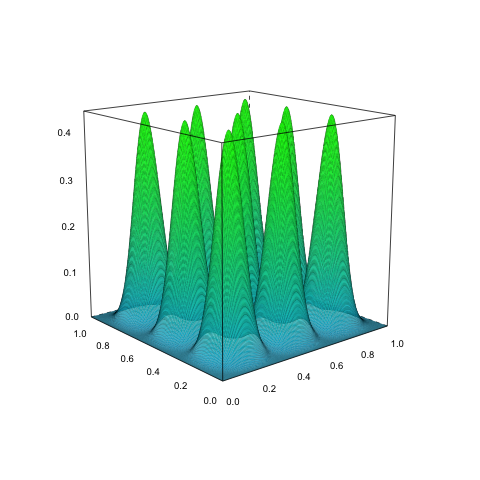
\includegraphics[width=4cm]{sparse_bicubic_basis}
% \caption{A ``thinned'' tensor product basis}
% \end{figure}
%     \end{center}
%\end{column}
%\end{columns}
%\vspace{0.3cm}
%\begin{equation*}
%\phi\left(l,m\right) = \sum_{i=1}^K \sum_{j=1}^L \theta_{ij} B_{i}\left(l\right) B_{j}\left(m\right)
%\end{equation*}
%
 
%The parameters of the functional autoregressive model given by \ref{eq:MyModel} define the elements of the precision matrix $\Omega$, rather than the elements of $\Sigma$ itself. It is well known that if we let $Y = \left(Y_1, \dots, Y_m\right)^\prime$ denote the random vector having joint distribution with mean zero and covariance matrix $\Sigma$, then the elements of $\Sigma^{-1}=\Omega$, $\left\{ \omega_{ij} \right\}$ may be interpreted as partial covariances between the elements of $Y$. This suggests shrinking $\phi$ to zero for large values of $l$. One can show that if $T$ has $k$ non-zero diagonals, then the middle $k$ diagonals of $\Sigma^{-1}$ are non-zero.  

%For ease of exposition, we first focus our attention on the estimation of $\phi$ assume that $\sigma^2\left(t\right)$ is fixed and known. Estimation of the innovation variance function is presented in Section~\ref{section:variance-estimation}. In the case that subjects share a common set of observation times $t_1 < \dots < t_m$,  it is well known that the MLE for $\Sigma$, $S = \sum_{i=1}^N y_i y_i^\prime$ is highly unstable in high dimensions, a condition that is potentially worsened when one or more subjects has at least one observation time that is unique from the set of observation times common across subjects. To mitigate instability due to high dimensionality and simultaneously permit the estimation of $\phi\left(\cdot,\cdot\right)$ as a smooth bivariate function, we obtain a covariance estimator by applying bivariate smoothing of the elements of the Cholesky factor. 
%
%Estimating the varying coefficient function $\phi$, however, is quite different from the usual problem of estimating an arbitrary bivariate function. In the case of the latter, we most typically treat both arguments equally in terms of regularization, but in the case of covariance estimation and the generalized coefficient function equal treatment of $l$ and $m$ in terms of penalization perhaps is not the most appropriate approach. The lag component, $l$, has particularly significant meaning in terms of the covariance function and thus also in terms of $\phi$ and is of considerable more interest than the orthogonal component, $m$. We parameterize $\phi$ in terms of the transformed domain:
%
%\begin{align*}
%l = t-s, \qquad m = \frac{1}{2}\left(s+t\right),
%\end{align*}
%\noindent
%so that the following relationship holds:
%\begin{align*}
%\phi\left(s,t\right) = \phi\left(s-t, \frac{1}{2}\left(s+t\right)\right) =\phi\left(l,m\right)
%\end{align*}
%with 
%\begin{equation} \label{eq:phi-star-domain}
%\frac{l}{2} < m < 1 - \frac{l}{2}, \quad 0 < l < 1.
%\end{equation}
%
%\noindent
%The likelihood can be written in terms of the reparameterized varying coefficient function:
%
%\begin{align} 
%\begin{split} \label{loglikelihood}
%-2L\left(y_1,\dots,y_N ,\phi \vert \vsigmasq \right) &= \sum_{i=1}^n \sum_{j=2}^{m_i} \sigma_{ij}^{-2} \left(y_{ij} - \sum_{k=1}^{j-1}\phi\left({t_{ij},t_{ik}}\right)y_{ik} \right)^2 \\
%&= \sum_{i=1}^n \sum_{j=2}^{m_i} \sigma_{ij}^{-2} \left(y_{ij} - \sum_{k=1}^{j-1}\phi\left({l_{ijk},m_{ijk}}\right)y_{ik} \right)^2 
%\end{split} 
%\end{align}

%%====================================================================================

\subsection{Model selection and tuning parameter estimation}

%\subfile{chapter-3-subfiles/chapter-3-tensor-product-pspline-model-selection}
\subsubsection{The limiting behaviour of $H_\lambda$}


The inspection of the hat matrix 

\[
H_\lambda = W B\left(W B^\prime W B +  \lambda_l P_l + \lambda_m P_m \right)^{-1} \left(W B\right)^\prime D^{-1}.
\]
\noindent
and its properties are integral for assessing model complexity and selecting the optimal values of the tuning parameters $\lambda_l$ and $\lambda_m.$  Summarizing the complexity of a fitted P-spline is far from a trivial task; one must simultaneously consider the value of the smoothing parameter, the number of basis functions in the B-spline basis, as well as the order of the difference penalties. We follow \cite{eilers1996flexible} and\cite{marx2005multidimensional} assess model complexity as discussed in cite{hastie1990generalized}, who proposed to use the trace of the smoother matrix as an approximation  to the effective dimensions of linear smoother. The \emph{effective dimension} is easily obtained and combines the effect of all three of these elements: 

%This approach to approximating the effective model dimension is also consistent with \cite{ye1998measuring}, who constructed a generalization of the concept of a model's degrees of freedom using the idea that the degrees of freedom can also be interpreted as the sum of the sensitivity of each fitted value with respect to the corresponding observed value.  For smoothing matrix $H$, the predicted response values are given by $\hat{y} = H y$. Writing
%
%\begin{align*}
%\frac{\partial \hat{y_i}}{\partial y_i} = \frac{\partial }{\partial y_i} \sum_{j} h_{ij} y_j = h_{ii},
%\end{align*}
%\noindent
%we see that the latter interpretation of the effective model dimension reduces to calculating the trace of the hat matrix. Thus we take the effective dimension to be 
%\begin{align}
%\textup{ED}\left(\lambda\right) &= \textup{tr}\left(H\right) \nonumber \\
%&= \textup{tr}\bigg[ B\left( B^T B + \lambda D^T D \right)^{-1} B^T\bigg], \label{eq:hat_matrix_trace}
%\end{align}

\begin{align}
\begin{split} \label{eq:hat-matrix-trace}
\textup{ED} &= \textup{tr} \left[ H_\lambda \right]\\
&= \textup{tr}\bigg[\left[WB \left(WB\right)^\prime D^{-1}WB +  \lambda_l P_l+ \lambda_m P_m\right]^{-1} \left(W B\right)^\prime D^{-1}  \bigg]
\end{split}
\end{align}
\noindent
When the number of basis functions is significantly smaller than the sample size, it is computationally advantageous to use the cyclic property of the trace: 

\begin{equation*}
\textup{tr}\bigg[\left[ \left(WB\right)^\prime D^{-1}WB +  \lambda_l P_l+ \lambda_m P_m\right]^{-1} \left(W B\right)^\prime D^{-1} WB  \bigg],
\end{equation*}
\noindent
which requires computing the trace of a $KL \times KL$ matrix. The effective dimension approaches $d_l + d_m$, the order of the differencing operator, as $\lambda$ increases, where $d_l$ and $d_m$ denote the orders of the difference penalties in the $l$ and $m$ directions, respectively.  Let
\begin{equation*}
Q = \left(W B\right)^\prime D^{-1} WB \qquad \mbox{and} \qquad Q_\lambda = P.
\end{equation*}

Using properties of the matrix trace, we can write
\begin{align*}
%\begin{split}
\mbox{tr}\left(H_\lambda \right) &= \mbox{tr}\bigg[ \left(Q + Q_\lambda \right)^{-1}Q \bigg]\\
&=\mbox{tr}\bigg[ Q^{1/2}\left(Q + Q_\lambda \right)^{-1}Q^{1/2} \bigg] \\
&=\mbox{tr}\bigg[\left(I + Q^{-{1/2}}Q_\lambda Q^{-{1/2}} \right)^{-1} \bigg]
%\end{split}
\end{align*}
Define $L \equiv Q^{-{1/2}}Q_\lambda Q^{-{1/2}}$. Then
\begin{equation*}
\mbox{tr}\left(H_\lambda \right) = \mbox{tr}\bigg[\left(I + \lambda L \right)^{-1} \bigg] = \sum_{j=1}^n \frac{1}{1 + \lambda \gamma_j}
\end{equation*}
 where $\gamma_j$, $j=1,\dots,n$ are the eigenvalues of $L$. $Q_\lambda$ has exactly $d_l + d_m$ eigenvalues equal to zero. Hence, $L$ has $d_l + d_m$ zero eigenvalues. For large $\lambda$, only the $d_l + d_m$ terms with $\gamma_j=0$ contribute to the sum which gives the trace of $H$, so that
 \[
\lim_{\lambda \rightarrow \infty  } \mbox{tr}\left(H\right) = d_l + d_m.
 \]

%A further simplification of \ref{eq:hat-matrix-trace}
%
%\begin{align*} 
%\left(B^T B + \lambda D^T D \right)^{-1} B^T B &= \left(B^T B + \lambda D^T D \right)^{-1} \left( B^T B + \lambda D^T D - \lambda D^T D\right) \nonumber \\
%&= I - \lambda\left(B^T B + \lambda D^T D \right)^{-1} D^T D \label{eq:cyclic_hat_matrix_simplification}
%\end{align*}
%
%\begin{align*} 
%\left[\left(WB\right)^\prime D^{-1}WB +  \lambda_l P_l+ \lambda_m P_m\right]^{-1} \left(W B \right)^\prime D^{-1} WB  &= \left[\left(WB\right)^\prime D^{-1}WB +  \lambda_l P_l+ \lambda_m P_m\right]^{-1}\left(W B \right)^\prime D^{-1} \times \\
%&\mbox{\;\;\;\;\;\;\;\;\;\;\;\;\;\;\;\;\;\;\;\;\;} \left[WB + \lambda_l P_l+ \lambda_m P_m - \left(\lambda_l P_l+ \lambda_m P_m\right) \right] \\
%&= I - \lambda\left(B^T B + \lambda D^T D \right)^{-1} D^T D \label{eq:cyclic_hat_matrix_simplification}
%\end{align*}

Equation~\ref{eq:cyclic_hat_matrix_simplification} cleanly shows that the effective dimension is always less than $n$, the number of B-spline used in the regression basis; further, the effective dimension is always smaller than $\min\left(m,n\right)$. A formal proof follows below. This is illustrated in 

Figure~\ref{fig:PS_ED_figure_1} shows how the effective dimension on a univariate P-spline changes with the smoothing parameter for the ten simulated observations in Figure~\ref{fig:overcomplete_basis_pspline} using 60 B-spline basis functions. For small $\lambda$, the effective dimension approaches $m$. As $\lambda$ increases, the effective dimension approaches the order of the difference penalty, $d$. It is worth pointing out here that there are no problems incurred when smoothing with many more B-splines than observations since the effective model dimension is always less than $m$, for all $\lambda$. 

\begin{figure}[H]
\begin{subfigure}{.5\textwidth}
  \centering
   \graphicspath{{img/}}
  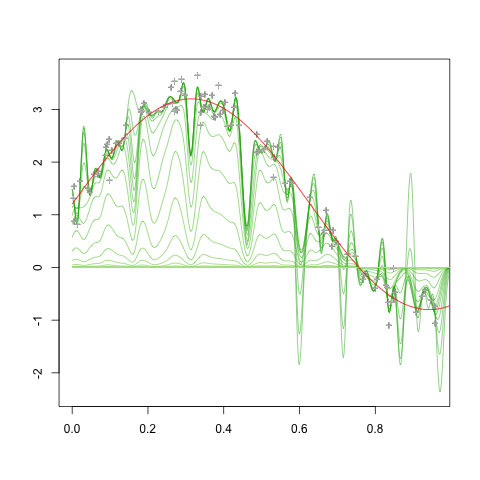
\includegraphics[scale=0.5]{PS_penalty_section_figure_6_order_0.png}
  %\label{fig:pspline_small_lambda}
\caption{$d=0$ }
\end{subfigure}
\begin{subfigure}{.5\textwidth}
  \centering
   \graphicspath{{img/}}
  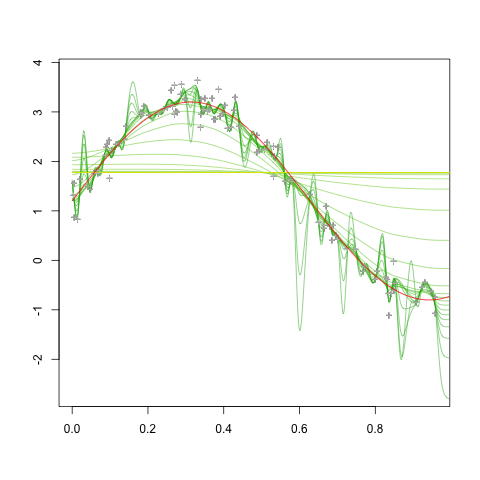
\includegraphics[scale=0.5]{PS_penalty_section_figure_6_order_1.png}
 % \label{fig:pspline_small_lambda}
\caption{$d=1$}
\end{subfigure}
\begin{subfigure}{.5\textwidth}
  \centering
   \graphicspath{{img/}}
  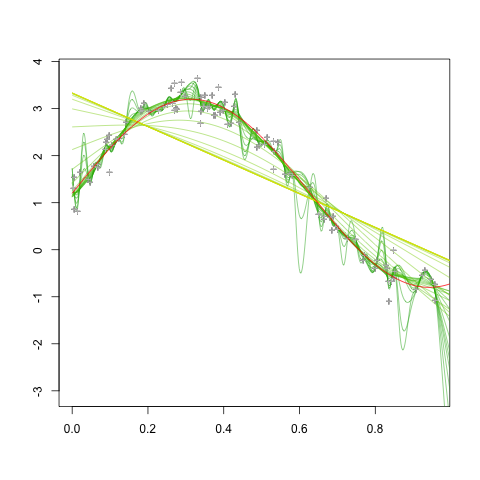
\includegraphics[scale=0.5]{PS_penalty_section_figure_6_order_2.png}
  %\label{fig:pspline_small_lambda}
\caption{$d=2$}
\end{subfigure}
\begin{subfigure}{.5\textwidth}
  \centering
   \graphicspath{{img/}}
  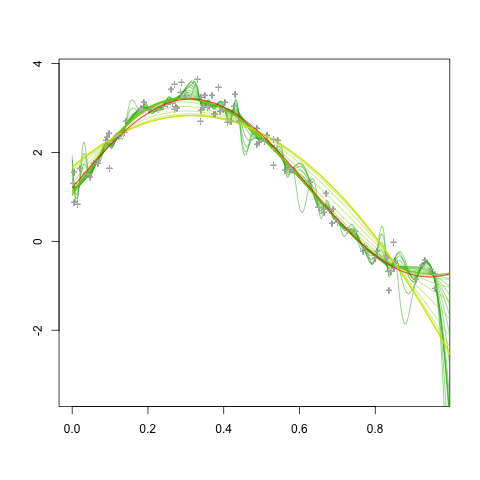
\includegraphics[scale=0.5]{PS_penalty_section_figure_6_order_3.png}
  %\label{fig:pspline_small_lambda}
\caption{$d=3$}
\end{subfigure}
\caption{\textit{Illustration of the impact of the order of the difference penalty. The number of B-splines used is the same in each plot, with the penalty parameter varying from across the same grid of values. The fitted curves in the upper left plot correspond to the difference penalty of order $0$, where $\vert D_0 \alpha \vert^2 = \sum_{i=1}^n \alpha_i^2$, analogous to ridge regression using the B-spline basis as regression covariates. The fitted curves approach polynomials of degree $d-1$ as $\lambda \rightarrow \infty$, as discussed in \ref{eq:PS_properties} \ref{eq:PS_property_3}.}}
\label{fig:PS_penalty_section_figure_6}
\end{figure}






